% FedECS-LT explained: a study text for the submitting author (docs/study/README.md, PROMPT.md).
% Every result number is a slot of the paper (\R{key}, ../papers/generated/numbers.tex), so the text follows the paper
% when new results arrive. Build: pdflatex fedecs_lt_explained.tex (three passes).
\documentclass[11pt,a4paper]{article}
\usepackage[T1]{fontenc}
\usepackage{lmodern}
\usepackage[a4paper,margin=2.7cm]{geometry}
\usepackage{microtype}
\usepackage{amsmath,amssymb,amsthm,mathtools}
\usepackage{graphicx}
\usepackage[export]{adjustbox}
\usepackage{booktabs}
\usepackage{xcolor,etoolbox,xspace}
\usepackage{tikz}
\usetikzlibrary{arrows.meta,positioning,calc,fit}
\usepackage{caption}
\captionsetup{font=small,labelfont=bf}
\usepackage[colorlinks,linkcolor=black,citecolor=black,urlcolor=black]{hyperref}
\usepackage[capitalise,nameinlink]{cleveref}
\crefname{section}{Chapter}{Chapters}
\crefname{subsection}{Section}{Sections}
\crefname{paragraph}{Section}{Sections}

\newtheorem{lemma}{Lemma}
\newtheorem*{lemma*}{Lemma}
\newcommand{\genpath}{../papers/generated}
% Shared macros of both versions of the paper (elsevier/main.tex, ieee/main.tex).
%
% RESULT SLOTS. Every number, table and figure that comes from an experiment is a slot. A slot shows a red
% placeholder until docs/papers/fill.py has written its value into docs/papers/generated/; then the value appears by
% itself. Never type a result into the text: run fill.py and rebuild (docs/papers/GUIDE.md).
%   \R{key}                    a number (generated/numbers.tex), e.g. \R{main/cifar10/FedECS-LT/bal}
%   \slottab{name}{fallback}   a tabular from generated/tables/name.tex; `fallback' (a placeholder tabular) until then
%   \slotfig{name}{size}{what} a figure from generated/figures/name.pdf; size = col (one column) or wide (page)
%   \claim{text}               a sentence whose wording depends on results: blue in draft mode, check it (GUIDE.md)
% \finalslotstrue in a wrapper turns every remaining placeholder into a LaTeX error, so that nothing unfilled is
% submitted.
\newif\iffinalslots
\makeatletter
\emergencystretch=2em   % placeholder names cannot be hyphenated
\providecommand{\genpath}{../generated}

\newcommand{\slotmissing}[1]{%
  \iffinalslots\PackageError{slots}{Result slot `#1' is not filled}{Run docs/papers/fill.py.}\fi
  \textcolor{red}{\textbf{[\detokenize{#1}]}}}

% numbers: generated/numbers.tex holds lines \defnum{key}{value}
\newcommand{\defnum}[2]{\expandafter\def\csname num@#1\endcsname{#2}}
\newcommand{\R}[1]{\ifcsname num@#1\endcsname\csname num@#1\endcsname\else\slotmissing{#1}\fi}
\InputIfFileExists{\genpath/numbers.tex}{}{}

% tables: the generated tabular, scaled down only if it is wider than the line
\newcommand{\slottab}[2]{%
  \IfFileExists{\genpath/tables/#1.tex}%
    {\begin{adjustbox}{max width=\linewidth}\input{\genpath/tables/#1.tex}\end{adjustbox}}%
    {\iffinalslots\PackageError{slots}{Table slot `#1' is not filled}{Run docs/papers/fill.py.}\fi
     \begin{adjustbox}{max width=\linewidth}#2\end{adjustbox}\par
     {\scriptsize\textcolor{red}{Placeholder: table slot \texttt{\detokenize{#1}} (GUIDE.md)}}}}
% one placeholder row: method name and n empty cells (the cells are built first, then emitted, so that the &s act
% as column separators of the table)
\newcommand{\phrow}[2]{\begingroup\count@=#2\relax\def\ph@c{}%
  \loop\ifnum\count@>\z@\edef\ph@c{\unexpanded\expandafter{\ph@c & --}}\advance\count@\m@ne\repeat
  \expandafter\endgroup\expandafter\ph@emit\expandafter{\ph@c}{#1}}
\newcommand{\ph@emit}[2]{#2#1\\}

% figures: the drawn PDF at its print size (column 3.5 in, page 7.16 in; IEEE format), never wider than the line
\newlength{\slotfigh}
\newcommand{\slotfig}[3]{%
  \IfFileExists{\genpath/figures/#1.pdf}%
    {\includegraphics[max width=\linewidth]{\genpath/figures/#1.pdf}}%
    {\iffinalslots\PackageError{slots}{Figure slot `#1' is not filled}{Run docs/papers/fill.py --figures.}\fi
     \ifstrequal{#2}{wide}{\setlength{\slotfigh}{0.28\textwidth}}{\setlength{\slotfigh}{0.55\linewidth}}%
     \fbox{\parbox[c][\slotfigh][c]{\dimexpr\linewidth-2\fboxsep-2\fboxrule\relax}{\centering\small
        \textcolor{red}{\textbf{FIGURE PLACEHOLDER: \texttt{\detokenize{#1}}}}\\[2pt]\footnotesize #3\par}}}}

% parts that exist only when their experiment came back: in draft mode always shown (with placeholders), in the
% final build (\finalslotstrue) left out when the result is missing, so that the paper never shows an empty slot.
%   \whentab{name}{...}  \whenfig{name}{...}  \whennum{key}{...}  \whenanytab{a,b,c}{...}
\newcommand{\whentab}[2]{\iffinalslots\IfFileExists{\genpath/tables/#1.tex}{#2}{}\else#2\fi}
\newcommand{\whenfig}[2]{\iffinalslots\IfFileExists{\genpath/figures/#1.pdf}{#2}{}\else#2\fi}
\newcommand{\whennum}[2]{\iffinalslots\ifcsname num@#1\endcsname#2\fi\else#2\fi}
\newif\ifslot@any
\newcommand{\whenanytab}[2]{\iffinalslots\slot@anyfalse
  \@for\slot@x:=#1\do{\IfFileExists{\genpath/tables/\slot@x.tex}{\global\slot@anytrue}{}}%
  \ifslot@any#2\fi\else#2\fi}

% a sentence to check against the results before submission (blue in draft mode, plain in final mode)
\newcommand{\claim}[1]{\iffinalslots#1\else\textcolor{blue}{#1}\fi}

% notation
\newcommand{\E}{\mathbb{E}}
\newcommand{\Rset}{\mathbb{R}}
\newcommand{\LSE}{\mathrm{LSE}}
\newcommand{\KL}{\mathrm{KL}}
\newcommand{\ER}{ER\xspace}
\newcommand{\ours}{FedECS-LT\xspace}
\newcommand{\geflf}{GeFL-F\xspace}
\newcommand{\pos}[1]{\textbf{#1}}
\makeatother

\finalslotstrue   % every number must be filled: a missing slot is an error

\setlength{\parskip}{0.35em}
\linespread{1.08}
\renewcommand{\paragraph}[1]{\par\medskip\noindent\textbf{#1.}\enspace}

\begin{document}

\begin{center}
{\Large\bfseries FedECS-LT, from the problem to the defence}
\end{center}
\medskip

\section{The problem}\label{ch:problem}

\paragraph{Federated learning} In federated learning, data stay on the devices or institutions that own them, the
\emph{clients}. A \emph{server} coordinates training. In each \emph{round} the server sends a model to the clients,
each client trains it for a while on its own data, and the server combines the returned models into a new one. The
standard way of combining is FedAvg: the server averages the clients' parameters, coordinate by coordinate. No raw
data leave a client; only parameters or other summaries do.

\paragraph{Different models} FedAvg needs every client to train the same network, because only then do the $j$-th
parameters of two clients mean the same thing. In practice clients run different hardware, so they may run different
networks: a phone runs a small convolutional network, a hospital server a larger one. This is
\emph{model-heterogeneous} federated learning. Parameters of different architectures cannot be averaged, so the
clients must share knowledge in another form. The paper studies one such form, a shared generator of synthetic
features (\cref{ch:gefl}).

\paragraph{Skewed and long-tailed labels} The second difficulty is in the labels. Two properties combine.
\begin{itemize}
\item \emph{Label skew}: clients hold different classes in different proportions. A client may have hundreds of images
of one class and none of another.
\item \emph{A global long tail}: over the whole federation, a few classes are frequent and many are rare.
\end{itemize}
The paper builds both in a controlled way. The class sizes follow
\[
n_c\propto\rho^{-c/(C-1)},\qquad c=0,\dots,C-1,
\]
so class $0$ is the largest, class $C-1$ the smallest, and the \emph{imbalance ratio} $\rho=n_0/n_{C-1}$ fixes how
steep the tail is. The paper uses $\rho=100$. Each class is then divided among the $K$ clients by a Dirichlet draw: for
class $c$ a vector of shares $(p_{1c},\dots,p_{Kc})$ is drawn from $\mathrm{Dirichlet}(\alpha,\dots,\alpha)$, and client
$k$ receives a fraction $p_{kc}$ of the class. A small concentration $\alpha$ gives very uneven shares; the paper uses
$\alpha=0.5$.

\paragraph{The running example} The text returns to one concrete case throughout: CIFAR-10-LT with $\rho=100$, $K=10$
clients and $\alpha=0.5$, split with seed 3. The run logs give its class sizes,
\[
(n_0,\dots,n_9)=(4800,\,4800,\,3620,\,2170,\,1301,\,779,\,467,\,280,\,168,\,100),
\]
18,485 training images in all. The profile asks for more than 4,800 images of classes 0 and 1, but CIFAR-10 has only
5,000 per class and 200 are held out for validation, so these two classes are capped. The realised ratio is
therefore $4800/100=48$, not 100. The paper still names the setting by its target ratio $\rho=100$ and gives the
realised ratio in its dataset table (\cref{tab:s-datasets}).

The rare class 9 shows what the split does to a rare class. Of its 100 images, client 7 holds 63. The other holders
have between 1 and 14 each, and clients 2 and 5 have none. (Clients are numbered 1 to 10 here; in the run logs they
are 0 to 9.) A class that is rare in the federation is held by few clients, and most of them see it only a few
times.

\paragraph{How the loss is measured} Plain accuracy hides what happens to rare classes. Take a model that recognises
classes 0--4 with recall 90\% and classes 5--9 with recall 10\%. On a test set with the training proportions above,
its accuracy is
\begin{align*}
&\frac{0.9\cdot(4800+4800+3620+2170+1301)+0.1\cdot(779+467+280+168+100)}{18485}\\
&\qquad=\frac{15021.9+179.4}{18485}\approx82\%,
\end{align*}
because the first five classes hold 90\% of the images. Yet the model fails on half of the classes. \emph{Balanced
accuracy} is the mean of the per-class recalls, here $(5\cdot0.9+5\cdot0.1)/10=50\%$: every class counts equally,
whatever its size. It is the paper's primary metric. The test sets of CIFAR-10 and CIFAR-100 are balanced (1,000 and
100 images per class), so there the two measures coincide; on the naturally imbalanced datasets they do not.

With ten client models, one per architecture, the paper reports the mean over the ten models of each model's balanced
accuracy,
\[
\text{balanced accuracy}=\frac1G\sum_{g=1}^{G}\frac1C\sum_{c=1}^{C}r_{gc},
\]
where $r_{gc}$ is the recall of class $c$ by the model of architecture $g$ and $G=10$ is the number of architectures.

\begin{table}[t]
\centering\small
\caption{The datasets as used in the paper (the paper's dataset table): number of classes, training images held by
the clients, test images, and the realised ratio between the largest and the smallest class. The first two are the
long-tailed benchmarks built with $\rho=100$; the others keep their own class sizes.}
\label{tab:s-datasets}
\slottab{datasets}{}
\end{table}

\paragraph{Two protocols} The paper tests its method in two settings.
\begin{itemize}
\item \emph{Different client models}, the setting the method is built for: ten clients, each with its own head
architecture, on the long-tailed benchmarks CIFAR-10-LT and CIFAR-100-LT and on six datasets whose classes are
naturally imbalanced (\cref{tab:s-datasets}).
\item \emph{One shared model}, the standard protocol of federated long-tail research: twenty clients train one
ResNet-8 together. Here the specialised long-tail methods of the literature apply, so this setting shows how the
method compares with them outside its own design.
\end{itemize}

The question the rest of this text builds on is how clients that run different models can share knowledge at all.

\section{The base system: GeFL-F}\label{ch:gefl}

Model-heterogeneous methods differ in what the clients exchange: predictions on shared inputs (FedDF, FedMD), class
means of internal representations (FedProto, FedTGP), a shared part of the network (LG-FedAvg, FedGH, FedMRL), or a
generator of synthetic data (FedGen, GeFL). The paper builds on GeFL-F, the feature-level variant of GeFL. It splits
every client's network into two parts, a small \emph{extractor} that all clients share and a \emph{head} that is
specific to the client's architecture, and lets the clients share a generator of extractor outputs. Training runs in
three stages (\cref{fig:s-pipeline}).

\begin{figure}[t]
\centering
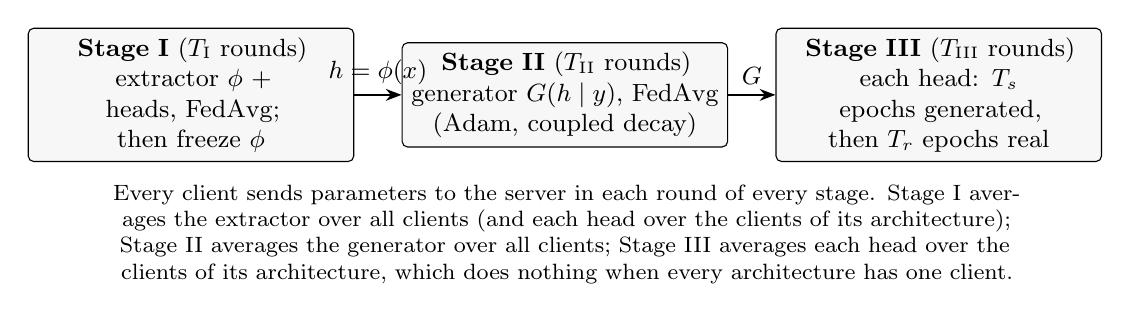
\begin{tikzpicture}[font=\small,
  box/.style={draw,rounded corners=2pt,align=center,minimum height=1.05cm,text width=3.9cm,fill=gray!6},
  arr/.style={-{Stealth[length=2mm]},thick}]
\node[box] (s1) {\textbf{Stage I} ($T_{\mathrm I}$ rounds)\\ extractor $\phi$ + heads, FedAvg;\\ then freeze $\phi$};
\node[box,right=0.6cm of s1] (s2) {\textbf{Stage II} ($T_{\mathrm{II}}$ rounds)\\ generator $G(h\mid y)$, FedAvg\\ (Adam, coupled decay)};
\node[box,right=0.6cm of s2] (s3) {\textbf{Stage III} ($T_{\mathrm{III}}$ rounds)\\ each head: $T_s$ epochs generated,\\ then $T_r$ epochs real};
\draw[arr] (s1) -- node[above]{$h=\phi(x)$} (s2);
\draw[arr] (s2) -- node[above]{$G$} (s3);
\node[below=0.35cm of s2,align=center,text width=12.5cm,font=\footnotesize] {Every client sends parameters to the
server in each round of every stage. Stage I averages the extractor over all clients (and each head over the clients of
its architecture); Stage II averages the generator over all clients; Stage III averages each head over the clients of
its architecture, which does nothing when every architecture has one client.};
\end{tikzpicture}
\caption{GeFL-F's three stages. The extractor and the generator are shared by all clients; the heads are not.}
\label{fig:s-pipeline}
\end{figure}

\paragraph{Stage I: the shared extractor} All clients train a small convolutional extractor $\phi$ together with
their heads by FedAvg, for $T_{\mathrm I}=50$ rounds on CIFAR. The extractor is the same network for everyone, so it
can be averaged. On CIFAR it is two $3\times3$ convolutions with three and ten output channels, each followed by
batch normalisation and ReLU, and a $2\times2$ max pooling. A $32\times32$ image becomes a $10\times16\times16$ array,
the \emph{feature} $h=\phi(x)$, with $d=2560$ numbers. After Stage I the extractor is frozen, and every client computes
the features of its images once, without augmentation. From then on, every client works on features, not images.

\paragraph{The heads} Client $k$ trains a head of its own architecture, one of ten convolutional networks CNN-1 to
CNN-10 with one to four convolutional blocks of different widths. Each head has two parts. Its \emph{body}, the
convolutional blocks, maps a feature $h$ to an \emph{embedding} $e$; its \emph{last layer} is linear and maps $e$ to
the $C$ logits $f=We+b$. In the main setting there are ten clients and client $k$ trains architecture $k$, so each
architecture has exactly one client.

\paragraph{Stage II: the shared generator} The clients train a conditional variational autoencoder $G(h\mid y)$ on
their features, again by FedAvg, for $T_{\mathrm{II}}=200$ rounds, with the Adam optimiser and coupled weight decay
(an L2 penalty $\lambda\|\theta\|^2/2$ added to the loss). The generator takes a class label $y$ and random noise $z$
and outputs a feature $\tilde h$ that should look like a real feature of class $y$. The label enters through a linear
projection of the one-hot vector $e_y$; the weights that multiply class $c$ form a vector $r_c$, the \emph{class row}.
The class rows are the only parameters of the generator that belong to one class: everything the generator knows that
distinguishes class $c$ from the others must pass through $r_c$.

\paragraph{Stage III: training the heads} For $T_{\mathrm{III}}=100$ rounds, every client trains its head in two
phases. In the \emph{synthetic phase} it draws labels uniformly over all $C$ classes, generates features for them, and
trains for $T_s$ epochs on these pairs with cross-entropy ($T_s=1$ in GeFL-F). In the \emph{real phase} it trains for
$T_r=5$ epochs on its own features. The server then averages the heads of each architecture. With one client per
architecture this averaging does nothing, so in the main setting the only knowledge a head receives from other
clients comes through the generator. This fact returns in \cref{ch:results,ch:defence}.

\paragraph{Why a generator helps} Client 2 of the running example holds no image of class 9. Its real phase can only
teach its head to separate the classes it holds. The synthetic phase can show the head features of class 9, made by a
generator that was trained partly on client 7's 63 images of that class. If the generated class-9 features look like
real ones, client 2's head learns class 9 without ever seeing a class-9 image. Whether they do look like real ones is
the central question of \cref{ch:diagnosis}.

\paragraph{What goes wrong} GeFL-F was designed and evaluated on balanced clients. Under the long tail of the running
example it reaches \R{main/cifar10/GeFL-F/bal} balanced accuracy on CIFAR-10-LT, about the level of Local, in which
every client trains alone (\R{main/cifar10/Local/bal}). On the tail classes, the 40\% least frequent (classes 6--9),
its recall is \R{main/cifar10/GeFL-F/tail}. On CIFAR-100-LT it reaches \R{main/cifar100/GeFL-F/bal}, against
\R{main/cifar100/Local/bal} for Local. Federation through the generator brings almost nothing.

Where, inside these three stages, are the rare classes lost?

\section{What federation can and cannot bias}\label{ch:sums}

Before locating the loss, one fact narrows the search. It is also the idea on which the whole method rests.

\paragraph{A client split is a pure label shift} The Dirichlet split of \cref{ch:problem} decides \emph{how many}
images of each class a client gets, but within a class it picks the images uniformly at random. So the class-9 images
of client 7 are a random subset of all class-9 images, and the same is true of every client and class. In symbols, the
distribution of an image given its class is the same on every client as on the pooled data,
\[
P_k(x\mid y)=P(x\mid y)\quad\text{for every client $k$ that holds class $y$.}
\]
Only the class proportions $P_k(y)$ differ. The extractor is shared, so the same holds for the features $h=\phi(x)$.

The consequence: any quantity that describes one class, such as the mean feature of class 9, its spread, or the best
weight vector for class 9 in a last layer, has the \emph{same target} on every client that holds the class and on the
pooled data. Federation cannot move that target. It can only make the estimate noisier, because each client sees fewer
samples, or slower to learn. So when a class-level quantity ends up \emph{biased} in a federated method, something in
the method's estimation procedure must have caused it.

\paragraph{Sums are exact} Many class-level quantities can be computed from sums. The mean feature of class $c$ is
\[
\mu_c=\frac{\sum_k S^{(1)}_{kc}}{\sum_k n_{kc}},\qquad S^{(1)}_{kc}=\sum_{i\in D_{kc}}h_i,
\]
where $D_{kc}$ is client $k$'s set of class-$c$ images and $n_{kc}$ its size. If every client sends its count $n_{kc}$
and its sum $S^{(1)}_{kc}$, the server obtains $\mu_c$ exactly, whatever the split. For class 9 of the running
example, client 7 sends 63 and the sum of its 63 features, client 9 sends 14 and the sum of its 14, and so on; the
server divides the total sum by the total count, 100, and gets the same mean it would get from the 100 images in one
place. The paper states this as a lemma.

\begin{lemma*}[partition invariance]
An estimator that is a function of a sum $S=\sum_k\sum_{i\in D_k}T(x_i,y_i)$, with $T$ fixed in advance, takes the same
value for every partition of the pooled data, and equals the centralised estimator.
\end{lemma*}

The proof is that addition does not depend on the order or grouping of its terms. The lemma is simple, and the paper
says that it is known for closed-form federated classifiers (Fed3R, AFL, FedCOF). Its use here is that it tells which
quantities a federated method can compute \emph{without} the bias of \cref{sec:s-routes}: those that are functions of
per-client sums. The class spread is one. With $S^{(2)}_{kc}=\sum_{i\in D_{kc}}\|h_i\|^2$,
\[
V_c=\frac{\sum_k S^{(2)}_{kc}}{n_c}-\|\mu_c\|^2=\E\big[\|h-\mu_c\|^2\,\big|\,y=c\big],
\]
the mean squared distance of a class-$c$ feature from the class mean, is also exact.

\paragraph{Secure aggregation} Sending per-client sums to the server would reveal each client's class counts and
feature sums. \emph{Secure aggregation} is a cryptographic protocol that lets the server learn the sum over clients of
vectors and nothing else about any single vector. The basic idea: every pair of clients agrees on a random mask; one
adds it to its vector, the other subtracts it; each masked vector looks random to the server, but in the sum the masks
cancel. The paper uses Flower's SecAgg+, a variant that tolerates clients dropping out.

The protocol works on integers, so each vector is divided by a public bound and quantised to 30 bits with unbiased
stochastic rounding. The error is at most $1.5\times10^{-8}$ of the bound per client and coordinate. Values beyond
eight times the bound would be clipped, and with fewer than three participants the protocol cannot run and the sum is
computed in clear. The paper calls the statistics \emph{exact} in this sense: exact up to this quantisation. The
bounds come from a small validation set that the server holds (200 images per class on CIFAR-10, held out from the
training data), never from the clients' data.

What secure aggregation does not hide is the sum itself. If a class is held by a single client, the federation-level
sum of that class is that client's sum. \Cref{ch:method} returns to what the released sums reveal.

\paragraph{How bias still enters}\label{sec:s-routes} If the targets cannot be biased by the split, a federated method can
still bias its estimate of them in four ways, which the paper examines.
\begin{enumerate}
\item \emph{The optimiser.} An optimiser can treat clients that lack a class differently from clients that hold it,
and averaging can then pull a class parameter away from its target.
\item \emph{Parameters tied to one client's prior.} A last-layer bias trained on one client's data learns that
client's class proportions, which are not the federation's.
\item \emph{What the synthetic data teach.} Training on generated features teaches whatever those features carry. If
they do not carry their label, the training teaches something else.
\item \emph{Sample size.} Nonlinear estimates, such as a spread or an inverse covariance matrix, are biased in small
samples. Class 9 has 100 images and features of dimension 2560: its covariance matrix cannot even be inverted.
\end{enumerate}
The paper does not claim that the list is complete. For example, drift of the shared extractor in Stage I, where the
extractor is trained by FedAvg on skewed data, is not covered.

Which of these routes actually hurt GeFL-F?

\section{Where GeFL-F loses the rare classes}\label{ch:diagnosis}

The paper finds a candidate loss on each of the first three routes of \cref{sec:s-routes}: the optimiser in Stage II,
the last layer in Stage III, and the synthetic data in Stage III. Each subsection below gives the intuition with the
running example, the precise statement, and what the runs show. The strength of the evidence differs between the
three, and the paper says so.

\subsection{The generator: coupled weight decay under Adam}\label{sec:s-decay}

\paragraph{The situation} In one round of Stage II, every client starts from the global generator, takes some local
Adam steps on its own features, and returns its copy; the server averages the copies. Consider the class row $r_9$ of
the running example on client 2, which holds no image of class 9. Client 2 never generates a class-9 feature during
training, so its data loss does not depend on $r_9$ at all. The only force on $r_9$ is the weight decay. With coupled
decay the penalty $\frac\lambda2\|\theta\|^2$ is part of the loss, so the gradient of client 2's loss with respect to
$r_9$ is exactly
\[
g=\lambda r_9 .
\]
With plain SGD this would move $r_9$ by $\eta\lambda r_9$ per step, a tiny amount: with the generator's learning rate
$\eta=10^{-3}$ and decay $\lambda=10^{-3}$, one part in a million of the row per step. Adam behaves very differently.

\paragraph{Why Adam makes the decay large} Adam divides each gradient coordinate by a running estimate of its own
magnitude. With the running means $m$ of the gradient and $v$ of its square (decay rates $\beta_1=0.9$,
$\beta_2=0.999$) and their bias-corrected versions $\hat m,\hat v$, a step is
\[
\theta\leftarrow\theta-\eta\,\frac{\hat m}{\sqrt{\hat v}+\epsilon}.
\]
Take one coordinate of $r_9$ equal to $0.5$, so $g=\lambda\cdot0.5=5\times10^{-4}$. On the first step $m=0.1\,g$ and
$v=0.001\,g^2$; the bias corrections divide them by $1-0.9$ and $1-0.999$, so $\hat m=g$ and $\hat v=g^2$. The step is
$\eta\,g/(|g|+\epsilon)\approx\eta=10^{-3}$, in the direction of the sign of the coordinate. Now repeat with a decay
100 times smaller, $\lambda=10^{-5}$: then $g=5\times10^{-6}$, still much larger than $\epsilon=10^{-8}$, and the step is
again $\approx10^{-3}$. Adam's step does not depend on the size of the gradient, only on its sign and consistency. A
client that lacks class 9 therefore moves every coordinate of $r_9$ toward zero by about one learning rate per step,
whatever the decay, 2,000 times faster than SGD would in this example.

\begin{lemma*}[coupled decay under Adam]
On a client without class $c$, the gradient of the loss with coupled L2 regularisation $\lambda$ with respect to $r_c$
is exactly $\lambda r_c$. Since Adam is invariant to a positive rescaling of the gradient sequence up to its $\epsilon$,
each step of such a client moves every coordinate of $r_c$ toward zero by about the learning rate $\eta$, independently
of $\lambda$, as long as $\lambda|r_{c,j}|\gg\epsilon$. With $\lambda=0$ this shrinkage vanishes; with decoupled weight
decay (AdamW) it becomes a factor $1-\eta\lambda$ per step, which is negligible here.
\end{lemma*}

Two remarks complete the picture. A client keeps its Adam state between rounds while its parameters are reset to the
global ones, so a single step can be somewhat larger than $\eta$. And the effect is specific to \emph{federated}
training: on pooled data, every batch that contains class 9 gives $r_9$ a data gradient, Adam's estimate $v$ of the
squared gradient is dominated by these, and the decay stays small. This holds as long as class-9 batches come within
the memory of $v$, about $1/(1-\beta_2)=1000$ steps.

\paragraph{The holders do not compensate} One might expect the clients that hold class 9 to push $r_9$ back. They
push it toward a good value, not toward a larger norm: their data gradient fits the row and need not lengthen it. They
also see class 9 rarely. Stage II trains the generator for 5 local epochs per round in batches of 64 (from the code).
Client 1 of the running example holds 4 class-9 images among 913, so at most 4 of its 15 batches per epoch, and at most
20 of its 75 steps per round, contain the class. On every other step its gradient on $r_9$ is again only the decay
$\lambda r_9$, and Adam shrinks the row exactly as on a client without the class. So most holders shrink a rare class's
row most of the time.

\paragraph{Averaging turns this into contraction} After the round, the server averages the returned rows. Let
$\Delta_k=\|r_{k,9}\|-\|r_9\|$ be the change of the row's length on client $k$, $\bar G$ the mean change over the
holders, $\bar D$ the mean shrinkage over the non-holders, and $p=m/K$ the share of clients that hold the class.

\begin{lemma*}[contraction under flat averaging]
Under $r_c^+=\frac1K\sum_k r_{k,c}$, $\|r_c^+\|\le\|r_c\|+p_c\bar G_c-(1-p_c)\bar D_c$, with equality if and only if all
$r_{k,c}$ are non-negative multiples of one another. The row contracts whenever $p_c<\bar D_c/(\bar G_c+\bar D_c)$.
\end{lemma*}

The proof is the triangle inequality: the length of an average is at most the average of the lengths. The
inequality is often strict, because clients that fit class 9 to their own few images move the row in different
directions, and averaging vectors that point in different directions shortens them further. For a feel of the
numbers: if eight holders lengthen the row by $0.02$ each and two non-holders shorten it by $0.05$, the bound allows a
gain of $0.8\cdot0.02-0.2\cdot0.05=0.006$. If the holders' average change is zero, which is plausible when they rarely
see the class, the row shrinks by at least $0.2\cdot0.05=0.01$ every round, over 200 rounds.

The paper also gives a predictor of the direction, counting Adam steps:
\[
\kappa_c=\frac{\sum_{k\in H_c}q_k f_{kc}}{\sum_{k\notin H_c}q_k},
\]
where $H_c$ is the set of holders, $q_k$ the number of local steps of client $k$, and $f_{kc}$ the probability that a
batch of client $k$ contains class $c$. The numerator counts the steps on which a holder actually sees the class, the
denominator the steps on which a non-holder decays it. When $\kappa_c<1$ the row drifts toward zero. The paper is
explicit that this is a heuristic, not a bound: it ignores the momentum Adam carries between rounds, and it was
\emph{not} checked against the measured rows.

\paragraph{The remedies} Two changes remove the effect. Decoupled weight decay (AdamW) applies the decay outside
Adam's normalisation, so the shrinkage becomes the negligible factor $1-\eta\lambda$. Or the rows can be averaged over
their holders only, weighted by how much of the class each holds (class-count weighted averaging, CCWA, in
\cref{sec:s-gen}): the non-holders' term $\bar D$ then drops out of the lemma.

\paragraph{What was measured} The paper's figure of the class rows (\cref{fig:s-rows}) shows that after Stage II the
rows of the rarest classes are several times shorter than those of the most frequent ones. That is the predicted
effect. It is not yet evidence that the shrinkage \emph{causes} the rare classes' low accuracy, and the paper says
so, for a reason that comes from a second measurement.

After Stage I the server trains a classifier, the \emph{referee}, on the features of its validation images, and asks
it to classify 300 generated features of each class. The share it assigns to the intended class is the generator's
\emph{fidelity} for that class. If the decay were what makes rare classes fail, the rare classes' fidelity would be
low and the frequent classes' high. Instead GeFL-F's generated CIFAR-10-LT features are recognised at
\R{main/cifar10/GeFL-F/fidelity_all} on average (chance is 10\%), \R{main/cifar10/GeFL-F/fidelity_head} on the head
classes and \R{main/cifar10/GeFL-F/fidelity_tail} on the tail classes. On CIFAR-100-LT the mean is
\R{main/cifar100/GeFL-F/fidelity_all}, chance level (\cref{tab:s-fidelity}). GeFL-F's generator carries little class
information for \emph{any} class. The row shrinkage is a measured property of the generator; whether it causes the
rare-class loss is open. The direct test is GeFL-F with AdamW and nothing else changed, one of the runs not yet
returned (\cref{ch:results}). The referee's accuracy on held-out real features was not logged, so the fidelity values
compare generators with each other, not with real data.

\begin{figure}[t]
\centering
\includegraphics[width=0.62\linewidth]{\genpath/figures/fig_rows.pdf}
\caption{The paper's figure of the class rows: length of each class row of GeFL-F's generator after Stage II, classes
from the most frequent (left) to the least frequent (right); CIFAR-10-LT, mean over seeds 3--5. Look at how the
length falls toward the rare classes.}
\label{fig:s-rows}
\end{figure}

\begin{table}[t]
\centering\small
\caption{The paper's fidelity table: the referee's per-class accuracy on generated features (\%), averaged over all
classes and over the head (30\% most frequent), medium and tail (40\% least frequent) classes; mean $\pm$ standard
deviation over seeds 3--5. FedDF uses GeFL-F's generator. FedECS-LT's rows belong to \cref{ch:method}.}
\label{tab:s-fidelity}
\slottab{fidelity}{}
\end{table}

\subsection{The last layer: logit corrections cannot add information}\label{sec:s-lastlayer}

\paragraph{The situation} In Stage III, client 2's head is trained on client 2's features only, in the real phase.
Its last layer therefore learns client 2's class proportions: classes it holds often get large biases, the classes
it lacks (class 9 among them) get pushed down by every cross-entropy step, because cross-entropy lowers the logits of
all wrong classes. The natural fix from long-tail learning is to correct the loss with the client's class
frequencies. \emph{Logit adjustment} trains with $\ell(f+\tau\log\hat\pi_k,\,y)$, where $\hat\pi_k$ is client $k$'s
class distribution (with add-one smoothing, so that absent classes get a small non-zero frequency) and $\tau=1$.
Balanced Softmax and FedLC are of the same form: a constant vector $a_k$ added to the logits during training.

\begin{lemma*}[logit corrections are reparametrisations]
Let a head have a free last-layer bias $b$, trained by SGD without decay on $b$, and let $a_k\in\Rset^C$ be a constant
of client $k$, as in logit adjustment ($a_k=\tau\log\pi_k$), FedLC or Balanced Softmax. Training with the loss
$\ell(f+a_k,y)$ from $(\theta_0,b_0)$ produces exactly the trajectory of training with $\ell(f,y)$ from
$(\theta_0,b_0+a_k)$: every parameter except $b$ is the same at every step. FedRS, which scales the logits of absent
classes by $\alpha\in(0,1]$, is cross-entropy in the rescaled last-layer variables $\alpha w_c,\alpha b_c$ of those
classes, trained with the smaller learning rate $\alpha^2\eta$.
\end{lemma*}

The proof: $f+a_k=We+(b+a_k)$, and moving from $b$ to $b+a_k$ is a translation, which does not change gradients. So
training with the corrected loss is plain training that starts from the bias $b_0+a_k$; at test time the correction is
not applied, which amounts to subtracting $a_k$ from the logits. This is exactly \emph{post-hoc logit adjustment} of a
head trained from a shifted starting bias.

\paragraph{A three-class example} A client holds 70 images of class A, 30 of class B and none of class C. With add-one
smoothing its frequencies are $(71,31,1)/103$, so $a=\log\hat\pi\approx(-0.37,\,-1.20,\,-4.63)$. At test time the
corrected head adds $+4.63$ to class C's logit relative to plain training, $+3.43$ more than to class B. That raises
class C for \emph{every} input by the same amount. It cannot make class C high for images of class C and low for others,
because the weight vector $w_C$ never received a single gradient that points toward class-C features: the client has
no class-C features. The correction moves a threshold; it adds no information about the class. The body of the head
can still learn a somewhat different representation, because the shifted logits change the gradients that reach it,
but nothing tells it what class C looks like. A head trained on one client is an extreme case of what the literature
calls minority collapse: for the classes the client lacks, the imbalance ratio is infinite.

\paragraph{What follows} A last layer that knows the absent classes needs information from other clients. The
partition-invariance lemma of \cref{ch:sums} says where to get it: a last layer that is a function of sums over all
clients equals the one computed on pooled data. The paper's answer is the \emph{exact readout} of \cref{sec:s-readout},
a classifier computed from summed embedding statistics.

\paragraph{What was measured} Two measurements support this part of the diagnosis, and they are the strongest
evidence in the paper's analysis. First, replacing GeFL-F's trained last layers by the exact readout, with nothing else
changed, raises its balanced accuracy by \R{main/cifar10/GeFL-F/gain_er} points on CIFAR-10-LT and
\R{main/cifar100/GeFL-F/gain_er} on CIFAR-100-LT. Most of what GeFL-F loses is in the last layer. Second, the lemma
predicts that Balanced Softmax, FedLC and FedRS differ only in their last layers. Once these are replaced by the same
readout, the three methods reach \R{main/cifar10/Balanced Softmax/er_bal}, \R{main/cifar10/FedLC/er_bal} and
\R{main/cifar10/FedRS/er_bal} on CIFAR-10-LT, and \R{main/cifar100/Balanced Softmax/er_bal},
\R{main/cifar100/FedLC/er_bal} and \R{main/cifar100/FedRS/er_bal} on CIFAR-100-LT: the same, as predicted.

\subsection{The synthetic data: label-free features penalise the logit spread}\label{sec:s-spread}

\paragraph{The situation} In the synthetic phase, labels are drawn uniformly over the $C$ classes and the generator
makes a feature for each. If the generated feature carries its label, the head learns the class. If it does not, as
the fidelity of \cref{tab:s-fidelity} suggests for GeFL-F, the label is effectively independent of the feature, and
the training target is the uniform distribution.

\begin{lemma*}[label-free synthetic data]
If the synthetic label $y$ is uniform on $\{1,\dots,C\}$ and independent of the generated feature, then for every logit
vector $f$,
\[
\E_y\,\ell(f,y)=\LSE(f)-\bar f=\log C+\KL(u\,\|\,\mathrm{softmax}f)=\log C+\frac1{2C}\sum_c(f_c-\bar f)^2+O(\|f-\bar f\|^3),
\]
where $\LSE(f)=\log\sum_c e^{f_c}$, $\bar f$ is the mean logit and $u$ the uniform distribution.
\end{lemma*}

In words: averaged over the random label, the cross-entropy is smallest when all logits are equal, and it grows
roughly with the variance of the logits. Training on label-free features therefore pulls the logits together. The
paper measures this as the \emph{logit spread}: the mean over images of the standard deviation of a head's logits
across classes.

A numerical check with $C=10$: equal logits give the loss $\log10=2.303$. The logits $(2,0,\dots,0)$ give
$\LSE=\log(e^2+9)=2.797$ and $\bar f=0.2$, so the loss is $2.597$. The quadratic term alone predicts
$2.303+\frac1{20}(1.8^2+9\cdot0.2^2)=2.483$; the rest is the higher-order term. The more confident the head, the larger
the penalty, whatever the class.

\paragraph{What survives the alternation} The synthetic phase is followed by the real phase, which pushes the logits
apart again for the classes the client holds. The paper analyses the alternation in a simplified model with quadratic
losses (an appendix lemma). The round converges to a point where, along every direction of the parameters that the
real loss leaves free, the synthetic loss alone decides. For a head trained on one client, the directions that
concern its absent classes are almost free in this sense, so on them the label-free synthetic phase decides: it
flattens exactly the logits the client most needs. Not exactly free, because cross-entropy on the real data still
pushes the absent classes' logits down on data the head separates. Logit adjustment shifts those targets.

\paragraph{What was measured} The paper's figure of the logit spread (\cref{fig:s-spread}) shows, in every Stage-III
round on CIFAR-10-LT, that the synthetic phase reduces the spread of the heads' logits on the clients' real features,
and that it reduces it less for FedECS-LT than for GeFL-F. Two caveats keep this from being a clean test. FedECS-LT
also differs from GeFL-F in its number of synthetic epochs, its soft targets and logit adjustment, so the comparison
does not isolate the labels. And FedDF, which trains on GeFL-F's own label-free generator, loses \emph{less} spread
than FedECS-LT. So the size of the spread change is not determined by whether the generated features carry their
label. The lemma is exact; how much it matters in the real pipeline is not settled.

\begin{figure}[t]
\centering
\includegraphics[width=0.62\linewidth]{\genpath/figures/fig_spread.pdf}
\caption{The paper's logit-spread figure: change of the logit spread during the synthetic phase of each Stage-III
round (after minus before; negative means the logits were pulled together), CIFAR-10-LT, mean over clients and seeds
3--5. Look at the levels: GeFL-F lowest, FedECS-LT in between, FedDF highest.}
\label{fig:s-spread}
\end{figure}

What would a method look like that uses exact statistics exactly where these losses occur?

\section{FedECS-LT, component by component}\label{ch:method}

FedECS-LT (Exact Class Statistics for Long-Tailed federated learning) keeps GeFL-F's three stages and its frozen
extractor. It obtains the class-specific quantities of the generator and the last layer from statistics that secure
aggregation computes exactly (\cref{ch:sums}), the \emph{exact class statistics}, instead of from parameters
estimated by FedAvg. It also changes how the heads are trained, and it adds a last step that sets every last layer.
\Cref{fig:s-overview} is the paper's overview; this chapter takes the components in pipeline order.

\begin{figure}[t]
\centering
\includegraphics[width=\linewidth]{\genpath/figures/fig_overview.pdf}
\caption{The paper's overview of FedECS-LT. C: computed by each client; S: computed by the server; SA: summed over
the clients by secure aggregation. Read it left to right: statistics after Stage I, the generator chosen by the gate
(Stage II), the moment correction, the heads (Stage III), and the exact readout last.}
\label{fig:s-overview}
\end{figure}

\subsection{Statistics release}\label{sec:s-stats}

\paragraph{What it answers} Every later component needs the class means and spreads of the features. They are
functions of sums, so they can be computed exactly (\cref{ch:sums}).

\paragraph{How it works} After Stage I, client $k$ computes for every class $c$ its count $n_{kc}$, its feature sum
$S^{(1)}_{kc}$ and its sum of squared feature norms $S^{(2)}_{kc}$. Secure aggregation returns the totals, and the
server forms (\texttt{fedecs.moments\_from\_sums})
\[
\mu_c=S^{(1)}_c/n_c,\qquad V_c=S^{(2)}_c/n_c-\|\mu_c\|^2 .
\]
$\mu_c$ is the mean feature of class $c$, a vector of $d=2560$ numbers, and $V_c$ its \emph{spread}, the mean squared
distance of a class-$c$ feature from $\mu_c$. In this text ``spread'' without a qualifier always means $V_c$, a squared
quantity; the \emph{logit spread} of \cref{sec:s-spread} is a different measurement.

\paragraph{Cost} Each client sends $C(d+2)$ numbers once: for each class, one count, one number for the sum of squared
norms, and $d$ for the feature sum. On CIFAR-10 that is $10\cdot2562=25{,}620$ numbers.

\subsection{The generator}\label{sec:s-gen}

\paragraph{The mean-anchored generator} This is the default branch. It generates a class-$y$ feature as
\[
\tilde h=\mathrm{ReLU}\big(\mu_y+\mathrm{dec}(z,\,A\mu_y)\big),\qquad z\sim\mathcal N(0,I),
\]
where $\mathrm{dec}$ is the decoder network and $A$ a projection shared by all classes. The exact mean $\mu_y$ is
added directly, and the decoder only has to model the deviation from it. The class enters only through the vector
$\mu_y$, which the server computed exactly, and through $A$, which every class shares. The generator therefore has no
class row and no other class-specific parameter: the contraction of \cref{sec:s-decay} has nothing to shrink. It is
trained by FedAvg with Adam, like GeFL-F's.

\paragraph{What an anchor can express} An anchored generator can make two classes only as different as their means
allow. The paper's appendix bounds the difference by the \emph{Wasserstein distance} $W_1$ between the two generated
distributions, the least average distance by which the points of one must be moved to turn it into the other:
\[
W_1(G_c,G_{c'})\le(1+L\|A\|_2)\,\|\mu_c-\mu_{c'}\|,
\]
where $L$ is the Lipschitz constant of the decoder in its second input (how much its output can change per unit change
of $A\mu$) and $\|A\|_2$ the largest stretch of the projection. The proof idea: generate both classes from the same
noise $z$; then each generated pair differs by at most $\|\mu_c-\mu_{c'}\|$ from the anchor plus $L\|A\|_2$ times that
from the decoder, and the ReLU never increases a distance. In words: when two class means are close, the anchored
generator cannot make the classes far apart unless $L\|A\|_2$ is large, and nothing in training controls that factor.
GeFL-F's class rows have no such limit, because a class row can encode a difference between classes that the mean does
not show.

\paragraph{The separation gate} So the server first measures how separated the means are, relative to the spread
(\texttt{fedecs.separation\_F}):
\[
F=\frac{\frac1C\sum_c\|\mu_c-\bar\mu\|^2}{\frac1C\sum_c V_c},\qquad \bar\mu=\frac1C\sum_c\mu_c .
\]
The numerator is the spread of the class means around their centre, the denominator the average spread within a
class. (It is a form of the ratio that linear discriminant analysis maximises, which \cref{sec:s-readout} explains.)
If $F\ge F_0=0.05$, the server uses the mean-anchored generator; otherwise it falls back to GeFL-F's generator, with
class rows averaged by CCWA. The threshold was fixed during the method's development and not swept.

A toy case: two classes on a line with means $-1$ and $+1$, each with spread $V=4$ (standard deviation 2). Then
$\bar\mu=0$, the numerator is $(1+1)/2=1$, the denominator $4$, and $F=0.25$. Over pairs of distinct classes, two
class means are on average $\sqrt{2FC/(C-1)}$ root-mean-square spreads apart (an appendix identity): here
$\sqrt{2\cdot0.25\cdot2}=1$, and indeed the means are 2 apart and the spread's root is 2. The threshold $F_0=0.05$ with
ten classes means $\sqrt{2\cdot0.05\cdot10/9}\approx0.33$: class means a third of a spread apart. The running example
has $F\approx0.080$ (seed 3, run log), so two CIFAR-10 class means are on average about 0.42 spreads apart: in the
frozen feature space the classes overlap heavily, and yet the anchor branch is chosen. Across all the paper's runs $F$
ranges from \R{gate/F/min_all} to \R{gate/F/max_all}, and the gate chose class rows on \R{gate/rows_all} (the
shared-model protocol is described in \cref{ch:design}).

\paragraph{The fallback: class rows with CCWA} When the gate finds the means too close, the generator keeps GeFL-F's
class rows, but the server averages each row only over the clients that hold the class, weighted by how much of it
they hold:
\[
r_c\leftarrow\frac{\sum_k E(n_{kc})\,r_{k,c}}{\sum_k E(n_{kc})},\qquad E(n)=\frac{1-\beta^n}{1-\beta},\quad\beta=0.999 .
\]
$E(n)$ is the \emph{effective number of samples} (a function of a count, not the expectation $\E$), and this $\beta$
is CCWA's own constant, unrelated to Adam's $\beta_2$ although equal in value. $E(n)$ is zero for a client without the
class, so non-holders drop out and the term $\bar g^{-}_c$ of the contraction lemma disappears. It is close to $n$ for small
$n$ and saturates at $1/(1-\beta)=1000$, so one large client cannot dominate a class. For class 9 of the running
example, client 7 (63 images) gets weight $E(63)\approx61.1$, client 1 (4 images) gets $E(4)\approx4.0$, and clients 2
and 5 get zero. For class 1, client 7's 2,803 images give $E(2803)\approx940$, not 2,803. Both sums are computed by
secure aggregation, so the server never sees a single client's counts.

\subsection{Moment correction}\label{sec:s-mc}

\paragraph{What it answers} Even a generator anchored to the right mean can produce features with the wrong spread,
too concentrated or too dispersed, and a class-rows generator can drift in mean too. The server knows the exact mean
$\mu_c$ and spread $V_c$, so it can correct the generated features to match them.

\paragraph{How it works} After Stage II the server draws 500 features per class from the generator, measures their
mean $\tilde\mu_c$ and spread $\tilde V_c$, and from then on corrects every generated feature of class $c$ by
(\texttt{fedecs.MomentCalibratedGen})
\[
\tilde h\leftarrow\mathrm{ReLU}\big(\mu_c+s_c(\tilde h-\tilde\mu_c)\big),\qquad
s_c=\mathrm{clip}\Big(\sqrt{V_c/\tilde V_c},\;0.1,\;10\Big).
\]
The map first moves the generated class to its exact mean, then rescales the deviations so that their spread becomes
the exact one. One scale $s_c$ multiplies every coordinate, so the correction matches the total spread, not the shape
of the class: a class that is too wide in one direction and too narrow in another keeps that imbalance.

\paragraph{A worked example} Take one coordinate, for illustration, with exact mean $0.5$ and exact spread $0.25$,
and generated features of mean $0.8$ and spread $0.0625$. Then $s_c=\sqrt{0.25/0.0625}=2$. A generated value $0.7$
becomes $0.5+2(0.7-0.8)=0.3$; a generated value $0.5$ becomes $0.5+2(0.5-0.8)=-0.1$, which the ReLU sets to $0$. Before
the ReLU the corrected values have exactly the target mean and spread. The ReLU raises the negative ones to zero, which
pulls them toward the mean, so the corrected spread comes out a little below the target.

\paragraph{Why this map} Without the final ReLU and the clipping, this is the map that reaches the exact mean and
spread while moving the generated features as little as possible (an appendix lemma). The proof idea: for a map $M$
with the required mean and spread, the expected squared displacement $\E\|M(X)-X\|^2$ is fixed except for one term,
$-2\E\langle M(X)-\mu_c,\,X-\tilde\mu_c\rangle$, and the Cauchy--Schwarz inequality says this term is smallest when
$M(X)-\mu_c$ is a positive multiple of $X-\tilde\mu_c$, which is the map above. The ReLU keeps features non-negative, as
real features after a ReLU are, and the clipping prevents extreme rescaling, so in practice the moments match only
approximately. Across every class and run of the long-tailed benchmarks, the corrected spread is \R{main/mc_spread_lo}
to \R{main/mc_spread_hi} times the exact spread $V_c$ (median \R{main/mc_spread_med}), below one as the example
predicts.

\paragraph{Cost} The server sends $(\mu_c,\tilde\mu_c,s_c)$ to the clients once; each client holds the generator and
corrects its own samples.

\paragraph{What the evidence says} Matching moments is not the same as making features recognisable. The fidelity
table (\cref{tab:s-fidelity}) shows that on CIFAR-10-LT the correction raises the referee's accuracy on the head
classes from \R{main/cifar10/FedECS-LT/fidelity_head} to \R{main/cifar10/FedECS-LT/fidelity_mc_head}, and changes the
tail classes' from \R{main/cifar10/FedECS-LT/fidelity_tail} to \R{main/cifar10/FedECS-LT/fidelity_mc_tail} and the
mean from \R{main/cifar10/FedECS-LT/fidelity_all} to \R{main/cifar10/FedECS-LT/fidelity_mc_all}. The tail and mean
changes are within one standard deviation over the seeds. On CIFAR-100-LT the mean is unchanged
(\R{main/cifar100/FedECS-LT/fidelity_all} and \R{main/cifar100/FedECS-LT/fidelity_mc_all}). The component ablation
(\cref{sec:s-ablations}) finds no benefit for accuracy: the full method minus its variant without the correction is
\R{comp/cifar10/w/o moment correction/er_drop} points with the readout on CIFAR-10-LT.

\subsection{The heads}\label{sec:s-heads}

Each Stage-III round, client $k$, holding $n_k$ real images, first takes $T_s\lfloor n_k/B\rfloor$ SGD steps on batches
of $B$ corrected generated features ($B=128$ on CIFAR), that is, $T_s$ epochs of the size of its real data, and then
trains $T_r=5$ epochs on its real features. Each phase starts a fresh SGD optimiser (learning rate 0.1, no momentum).
Three things differ from GeFL-F.

\paragraph{Logit adjustment in the real phase} The real phase uses $\ell(f+\tau\log\hat\pi_k,y)$ with $\tau=1$ and the
client's add-one smoothed class frequencies $\hat\pi_k$. On a head trained only on real data this would add no
information about absent classes (\cref{sec:s-lastlayer}), but here it is applied in the real phase only, between
synthetic phases without it, so the reparametrisation lemma does not cover it. The paper gives two reasons for it:
without it, cross-entropy keeps pushing the absent classes' logits down during the real phase (\cref{sec:s-spread}),
and it can change what the body learns. $\hat\pi_k$ is the client's own frequencies, not an exact class statistic. How
much logit adjustment contributes is not resolved: its ablation finished one seed per benchmark
(\cref{sec:s-ablations}).

\paragraph{Consensus soft labels in the synthetic phase} The synthetic phase still draws labels uniformly, but the
target is no longer the one-hot label alone. For a generated feature $\tilde h$ with label $y$,
\[
t(\tilde h)=(1-\omega)\,\mathbf 1_y+\omega\,\frac1{10}\sum_{g=1}^{10}\mathrm{softmax}\big(f_g(\tilde h)\big),\qquad\omega=0.5,
\]
where $\mathbf 1_y$ is the one-hot vector of $y$ and $f_g$ the current head of architecture $g$. The second term is the
federation's averaged prediction on that feature, the same kind of target as FedDF's distillation. If a generated
``class 9'' feature looks to the federation's heads like class 3 with probability 0.4 and like class 9 with 0.05, its
target puts $0.5+0.5\cdot0.05=0.525$ on class 9 and $0.2$ on class 3. The weight $\omega=0.5$ was fixed in development.

This answers the third loss of \cref{ch:diagnosis}: the target now depends on the feature, so the premise of the
label-free lemma, a label independent of the feature, no longer holds, and the synthetic phase need not pull the logits
together. The intent is that the target follows what the feature carries instead of forcing a label it may not
support, and that every head learns from the ensemble of all ten architectures; the ablation confirms that consensus soft labels
improve accuracy: removing them costs \R{comp/cifar10/w/o consensus soft labels/er_drop} points with the readout on
CIFAR-10-LT and \R{comp/cifar100/w/o consensus soft labels/er_drop} on CIFAR-100-LT, the one component effect the
ablation resolves (\cref{sec:s-ablations}).

\paragraph{How the consensus is computed} The average is computed by one secure sum per round. Every client
regenerates the same pool of generated features from a seed the server sends. Writing $\mathrm{arch}(k)$ for the architecture
of client $k$, it returns $w_k\,\mathrm{softmax}(f_{\mathrm{arch}(k)}(\tilde h))$ for every feature of the pool, with
$w_k=1/(10\cdot|\{j:\mathrm{arch}(j)=\mathrm{arch}(k)\}|)$, one over ten times the number of clients of its own architecture. The secure sum of
these is the average above. The pool is as large as the largest client's synthetic phase, $T_s\lfloor n_k/B\rfloor B$
(\texttt{fedecs.csl\_pool\_size}): in the running example, client 7 with 4,538 images gives
$10\cdot35\cdot128=44{,}800$ features, so every client returns $448{,}000$ numbers per round. For this every client also
receives every architecture's current head each round, which FedAvg within an architecture would not require.

\paragraph{Ten synthetic epochs} $T_s=10$ instead of GeFL-F's 1. This is more computation, not a statistic, and the
paper lists it as one of the method's changes.

\subsection{The exact readout}\label{sec:s-readout}

This component gets the most space, because \cref{ch:results} shows that it carries most of the gain.

\paragraph{What it answers} \Cref{sec:s-lastlayer} showed that a last layer trained on one client knows nothing about
the classes the client lacks, and that a last layer computed from sums over all clients equals the one computed on
pooled data. The exact readout is such a last layer: after Stage III, every architecture's trained last layer is
replaced by a classifier computed from aggregated statistics of the embeddings.

\paragraph{The classifier} Suppose the embeddings $e$ of each class $c$ are Gaussian with mean $\nu_c$ and a covariance
$\Sigma$ shared by all classes, and every class is equally likely. Then the most probable class for an embedding $e$
maximises the log-density of $e$ under class $c$,
\[
\log \mathcal N(e;\nu_c,\Sigma)=-\tfrac12(e-\nu_c)^\top\Sigma^{-1}(e-\nu_c)+\text{const}
= e^\top\Sigma^{-1}\nu_c-\tfrac12\nu_c^\top\Sigma^{-1}\nu_c-\tfrac12e^\top\Sigma^{-1}e+\text{const}.
\]
The term $-\frac12e^\top\Sigma^{-1}e$ is the same for every class, so it does not affect which class wins. What is left
is linear in $e$: the logit of class $c$ is $w_c^\top e+b_c$ with
\[
w_c=\Sigma^{-1}\nu_c,\qquad b_c=-\tfrac12\,\nu_c^\top\Sigma^{-1}\nu_c .
\]
This is linear discriminant analysis (LDA). The usual LDA adds $\log\pi_c$, the class prior, to $b_c$, which favours
frequent classes. Leaving it out makes the classifier \emph{class-balanced}: it treats every class as equally likely,
which is what balanced accuracy rewards. The classifier is the nearest class mean in the Mahalanobis distance
$(e-\nu_c)^\top\Sigma^{-1}(e-\nu_c)$, a distance that measures each direction in units of the spread along it. LDA's
directions are also those that maximise the ratio of the spread between class means to the spread within classes,
which is why the gate's $F$ was called a form of its ratio.

\paragraph{A two-dimensional example} Take two classes with means $\nu_A=(1,1)$ and $\nu_B=(0,0)$ and the shared
covariance $\Sigma=\mathrm{diag}(1,\,0.25)$: the second coordinate is four times less noisy than the first. Then
$\Sigma^{-1}=\mathrm{diag}(1,4)$, $w_A=(1,4)$, $b_A=-\frac12(1+4)=-2.5$, $w_B=0$, $b_B=0$, and class A wins when
$x+4y>2.5$. The nearest-mean rule would instead decide by $x+y>1$. For the point $e=(1.2,\,0.3)$ the nearest-mean rule
says A, since $1.5>1$, but LDA says B, since $1.2+1.2=2.4<2.5$. The point is far from A along the precise coordinate
and close to B there, and LDA trusts that coordinate more (\cref{fig:s-lda}).

\begin{figure}[t]
\centering
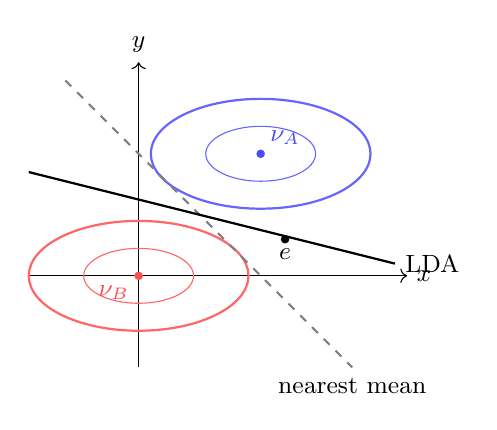
\begin{tikzpicture}[scale=1.55,font=\small]
\draw[->] (-0.9,0) -- (2.2,0) node[right]{$x$};
\draw[->] (0,-0.75) -- (0,1.75) node[above]{$y$};
\foreach \cx/\cy/\col in {1/1/blue!60,0/0/red!60}{
  \draw[\col,thick] (\cx,\cy) ellipse (0.9 and 0.45);
  \draw[\col] (\cx,\cy) ellipse (0.45 and 0.225);}
\fill[blue!70] (1,1) circle (0.035) node[above right]{$\nu_A$};
\fill[red!70] (0,0) circle (0.035) node[below left]{$\nu_B$};
\draw[gray,dashed,thick] (-0.6,1.6) -- (1.75,-0.75) node[below,black]{nearest mean};
\draw[black,thick] (-0.9,0.85) -- (2.1,0.1) node[right]{LDA};
\fill (1.2,0.3) circle (0.035) node[below]{$e$};
\end{tikzpicture}
\caption{Illustration of the readout's decision rule (made-up numbers, not data). Ellipses: equal-density contours of
two classes with a shared covariance that is narrow in $y$. Dashed: the nearest-mean boundary $x+y=1$. Solid: the LDA
boundary $x+4y=2.5$. Look at the point $e$: it is on A's side of the dashed line but on B's side of the solid one.}
\label{fig:s-lda}
\end{figure}

\paragraph{Shrinkage} In practice $\Sigma$ is estimated, and the embedding dimension is large: $d_e$ ranges from 80
(CNN-10) to 1024 (CNN-1) (\cref{tab:s-heads}). This is the fourth route of \cref{sec:s-routes}. Even with more images
(18,485 on CIFAR-10-LT) than dimensions, the smallest eigenvalues of an estimated covariance are systematically too
small, and since $\Sigma^{-1}$ divides by them, their errors dominate the classifier. The readout therefore uses
\[
\Sigma_\gamma=(1-\gamma)\Sigma+\gamma\,\frac{\mathrm{tr}\,\Sigma}{d_e}\,I,\qquad\gamma=0.1,
\]
a mix of the estimate with a multiple of the identity that has the same average variance, and sets
\[
w_c=\Sigma_\gamma^{-1}\nu_c,\qquad b_c=-\tfrac12\,\nu_c^\top\Sigma_\gamma^{-1}\nu_c
\]
(the paper's readout equation, \texttt{fedecs.lda\_from\_sums}). The paper's version uses a pseudo-inverse, and sets
$b_c=-10^4$ for a class that no client holds, so that it is never predicted.

Carried through the example, $\Sigma_\gamma=0.9\,\mathrm{diag}(1,0.25)+0.1\cdot0.625\,I=\mathrm{diag}(0.9625,\,0.2875)$,
so $w_A\approx(1.04,\,3.48)$ and $b_A\approx-2.26$. For $e=(1.2,0.3)$, $w_A^\top e=1.04\cdot1.2+3.48\cdot0.3\approx2.29$ now exceeds
$-b_A\approx2.26$, so A's logit is about $+0.03$, above B's logit $0$: with shrinkage the point goes back to A. Shrinkage pulls the
rule part of the way from LDA toward the nearest-mean rule, trusting the precise direction less, and with it the
estimates of the small variances, which are the least reliable part of the estimate.

\paragraph{How it is computed from sums} After Stage III the server sends every architecture's body to every client.
Each client passes its real features through every body and computes, per architecture, its per-class counts, the
per-class sums $\sum e$ of the embeddings, and the second moment $\sum ee^\top$. Secure aggregation sums them. From
these the server gets the class means $\nu_c$ and the pooled within-class covariance, which is the total second moment
minus $\sum_c n_c\nu_c\nu_c^\top$, divided by the number of images minus the number of classes. Everything is a
function of sums, so by partition invariance the readout equals the same estimator computed centrally on the pooled
embeddings of the same body. It is not the same as a last layer trained centrally by SGD.

\paragraph{What it is and is not} With the true means and covariance and $\gamma=0$, and if the embeddings really
were Gaussian with a shared covariance, this would be the Bayes classifier for equally likely classes. Computed from
data with shrinkage, it is a plug-in estimate of that classifier. When the embeddings are not Gaussian with a shared
covariance, which is the usual case, it is a linear classifier with no optimality guarantee. It belongs to a known
family of closed-form federated classifiers: Fed3R (a ridge-regression classifier), FedNCM (nearest class means) and
FedCOF (an LDA-type classifier with a covariance estimated from class means). What the paper adds is computing it
\emph{per architecture}, on bodies trained in the federation, with statistics from \emph{all} clients, including those
of other architectures. That is possible only because every client runs every architecture's body.

\paragraph{Where it helps and where it hurts} It helps most where a last layer was fitted to one client's prior, the
main setting. It changes FedECS-LT very little on OrganAMNIST and lowers it with one shared model, where the last layer
was trained by all clients; and its equal class priors lower the accuracy on each client's own class mix.
\Cref{ch:results} gives the numbers.

\paragraph{Cost} One extra round. Each client sends $C(d_e+1)+d_e^2$ numbers per architecture: $C$ counts, $C$
class sums of length $d_e$, and the $d_e\times d_e$ second moment. For CNN-1 with $d_e=1024$ the second moment alone is
about a million numbers. Every client must run a forward pass (no training) of every architecture's body on its own
features once; a client that cannot do so would be left out of the sums.

\paragraph{It can be added to other methods} The readout uses only a head's body, never its trained last layer, so it
can be added to any method whose heads have a body and a linear last layer. The \emph{methods of the GeFL-F pipeline}
are those that share GeFL-F's extractor and heads: GeFL-F, FedDF, Balanced Softmax, FedLC, FedRS and FedECS-LT. The
paper reports each of them both without the readout and with it added (``ER''), which separates the readout's gain from
the rest of each method. This is the comparison on which \cref{ch:results} turns.

\subsection{The whole recipe}\label{sec:s-recipe}

The paper's Algorithm 1 in words, one run:
\begin{enumerate}
\item \textbf{Stage I}: train the extractor $\phi$ and the heads by FedAvg; freeze $\phi$; every client computes
$h=\phi(x)$.
\item \textbf{Statistics release}: clients send $n_{kc},S^{(1)}_{kc},S^{(2)}_{kc}$ by secure aggregation; the server
forms $\mu_c,V_c$ and the gate $F$.
\item \textbf{Stage II}: if $F\ge F_0$, train the anchored generator by FedAvg; otherwise GeFL-F's generator with class
rows averaged by CCWA.
\item \textbf{Moment correction}: the server measures $\tilde\mu_c,\tilde V_c$ and sends $(\mu_c,\tilde\mu_c,s_c)$.
\item \textbf{Stage III}, for $T_{\mathrm{III}}$ rounds: the server sends the heads and a pool seed; the clients
return their predictions on the pool by secure aggregation, giving the consensus soft labels; each client trains
$T_s$ epochs on corrected generated features with consensus soft labels, then $T_r$ epochs on real features with logit
adjustment; the server averages heads of the same architecture.
\item \textbf{Exact readout}: clients send embedding sums per architecture by secure aggregation; the server sets
every last layer to the class-balanced LDA.
\end{enumerate}
The settings are the same on every dataset: $F_0=0.05$, $\beta=0.999$, 500 samples for the moment correction with
$s_c\in[0.1,10]$, $T_s=10$, $T_r=5$, $\tau=1$, $\omega=0.5$, $\gamma=0.1$; the generator uses Adam with learning rate
$10^{-3}$ and coupled decay $10^{-3}$, as in GeFL-F.

\paragraph{Which component uses what} Three steps use the exact class statistics: the anchored generator (or CCWA), the
moment correction, and the readout, which uses the corresponding statistics of the embeddings. Logit adjustment uses
the client's own frequencies, consensus soft labels use the heads' predictions, and $T_s=10$ is computation. The
method's name describes the first group.

\subsection{Cost and privacy}\label{sec:s-privacy}

Beyond GeFL-F, FedECS-LT sends the class statistics once, the moment correction once, the consensus predictions every
round, and the readout sums once. The measured totals are in \cref{ch:results}.

\paragraph{What is revealed} Secure aggregation hides each client's own vectors. The server, and through the generator
and the moment correction every client, learns the federation-level class means and spreads. For a class that one
client holds, these equal that client's own statistics. For a class with few images they reveal more about each image
than a mean over thousands would: each of class 9's 100 images enters its class mean with a weight of one hundredth. The features
come from a shallow extractor, two convolutions and a pooling, so a class mean is close to a mean image at half
resolution. The paper did not test how much of the images an inversion of the released means recovers. Formal
differential privacy, adding calibrated noise to the sums, is possible but not part of the results, and it would not
cover the FedAvg training of the generator and heads. The security model is an \emph{honest-but-curious} server, one
that follows the protocol but tries to learn what it can from what it receives; the paper says FedECS-LT should not be
called privacy-preserving beyond what secure aggregation guarantees against such a server. Every client also receives
every architecture's head (consensus) and body (readout), so the architectures are not secret, and every client must be
able to run the largest of them.

How is such a method tested, and against what?

\section{The study design}\label{ch:design}

The experiments have to show three things: that the losses of \cref{ch:diagnosis} occur, that FedECS-LT recovers
them, and which part of FedECS-LT does so. Every choice below serves one of these, or protects the comparison against
a way of being unfair.

\subsection{The research questions}\label{sec:s-rq}

\begin{itemize}
\item \textbf{RQ1, diagnosis.} Do the three losses occur in GeFL-F's own runs? Answered by the class rows, the readout
gain and the logit spread (\cref{ch:diagnosis}).
\item \textbf{RQ2, effect.} Does FedECS-LT, ending with its readout, raise balanced accuracy over GeFL-F and the other
model-heterogeneous methods, each as it is without the readout? Answered by the main comparison (\cref{sec:s-main}).
\item \textbf{RQ3, body or last layer.} How much of the difference remains when every method of the GeFL-F pipeline
gets the same readout, so that only the heads' bodies differ? Answered by the readout comparison
(\cref{sec:s-same-readout}).
\item \textbf{RQ4, scope.} Does the effect hold with natural class imbalance and in the protocol with one shared
model? Answered in \cref{sec:s-natural,sec:s-shared}.
\item \textbf{RQ5, components.} Which changes carry the effect? Answered by the ablations, whose runs are pending
(\cref{sec:s-pending}).
\end{itemize}
RQ3 is the question that decides how the paper's claim must be worded, as \cref{ch:results} shows.

\subsection{Datasets and splits}

\paragraph{The long-tailed benchmarks} CIFAR-10-LT and CIFAR-100-LT are built by the paper with $\rho=100$. GeFL-F
uses half of CIFAR-10's training set, so the profile is applied to that half (and to 22\% of CIFAR-100, which gives the
usual CIFAR-100-LT shape). As \cref{ch:problem} showed, the largest classes are capped, so the realised ratios are 48
and 96 (\cref{tab:s-datasets}). The class index orders classes from the most to the least frequent, so the tail
classes are the same in every run. MNIST, Fashion-MNIST and SVHN belong to the same benchmark set; their runs had not
returned when this text was written.

\paragraph{The naturally imbalanced datasets} Six datasets keep their own class sizes, with training sets capped at
20,000 images: DermaMNIST, OrganAMNIST, BloodMNIST and PathMNIST (medical images), EMNIST ByClass (handwritten
characters, 62 classes) and FER-2013 (facial expressions). Their realised ratios range from 2 to 75. On OrganAMNIST,
BloodMNIST and PathMNIST the ratio is 5 or less, so there the results speak to label skew more than to a long tail.
These six datasets were never used while the method was being developed, which makes them the cleanest evidence in
the paper.

\paragraph{Splits} Each class is divided among $K=10$ clients by a Dirichlet draw with $\alpha=0.5$. The draw is
repeated, at most 100 times, until every client holds at least ten images. A held-out block of training images that
no client holds, 200 per class on CIFAR-10, forms the server's validation set. It has two uses only: it trains the
referee of the fidelity measurement, and it sets the public bounds of secure aggregation. It is never used to select a
model or a setting. Every reported number is on the official test set. The paper checked that every client's class
counts are identical across methods for every dataset and seed.

\paragraph{Seeds} Every configuration runs with seeds 3, 4 and 5. A seed fixes the split and every method's
initialisation, so two methods with the same seed see exactly the same clients: their results are \emph{paired}.

\subsection{The two protocols}

\paragraph{Different client models} The main setting is GeFL-F's: 10 clients, one per architecture, with GeFL-F's
rounds ($T_{\mathrm I},T_{\mathrm{II}},T_{\mathrm{III}}=50,200,100$ on CIFAR). All federated methods of this setting
share the same Stage-I extractor for a given dataset and seed, so they differ only in what they do after Stage I.

\paragraph{One shared model} The second protocol is the one used by federated long-tail research, taken from the
FedLTLib benchmark, whose settings come from CReFF: CIFAR-10-LT and CIFAR-100-LT at $\rho=100$, 20 clients, 8 of them
(40\%) in each round, Dirichlet $\alpha=0.5$, one ResNet-8 shared by all, 200 rounds of 10 local epochs (batch 32, SGD
with learning rate 0.1, momentum 0.9, decay 0.99 per round). The baselines run their authors' LongTailLib code
unchanged on the paper's splits, with ResNet-8 for every method.

FedECS-LT is fitted into this protocol by splitting the ResNet-8 after its second stage into a frozen extractor and a
head. The extractor trains for 100 rounds, the generator for 100, and the head for 100 with 10 real epochs per round;
so FedECS-LT uses the baselines' 200 training rounds plus 100 generator rounds. Two differences matter later: its head
trains on frozen features of unaugmented images, while the baselines train the whole network end to end with
augmentation; and with a single architecture the consensus soft label is just the shared model's own prediction.

\subsection{The methods compared}\label{sec:s-methods}

Each group of methods answers a specific question.
\begin{itemize}
\item \textbf{GeFL-F}, the method FedECS-LT extends: the difference to it is the effect of the changes.
\item \textbf{FedDF}, ensemble distillation on the server: after each round the server distils every architecture
toward the ten architectures' mean prediction, for 20 steps. FedDF originally distils on public data; here it distils
on GeFL-F's generated features, so that no method uses data that no client holds. It is the strongest generator-based
competitor.
\item \textbf{Per-client long-tail losses}: Balanced Softmax, FedLC and FedRS, applied to the heads with \emph{no
generator}. They test whether correcting the loss alone repairs the long tail. By the reparametrisation lemma they
should behave alike, and \cref{ch:diagnosis} showed that they do once the readout is added.
\item \textbf{Model-heterogeneous methods from the HtFLlib library}: prototypes (FedProto, FedTGP), a generator of
embeddings (FedGen), a shared global head (FedGH), shared last layers (LG-FedAvg) and shared sub-networks (FedMRL). They
represent the other ways of sharing knowledge between different models. They were designed for label skew without a
global long tail and are ported to the frozen extractor with HtFLlib's settings.
\item \textbf{Local}: each client trains its extractor and head alone. It is the reference without federation.
\item \textbf{One-shared-model methods}: FedAvg, FedProx, MOON, FedLC, CCVR, CReFF, FedETF, Fed-GraB, FedLoGe, FedYoYo
and RUCR, in the second protocol only.
\end{itemize}
Two further groups, GeFL's own grouped baselines and a reference trained on all data pooled, are planned for GeFL's
50-client setting and had not returned when this text was written.

\paragraph{Fairness of the comparison} The paper's fairness table records what each method spends and exchanges.
FedECS-LT trains 10 synthetic epochs per round against 1 for GeFL-F and FedDF and none for the methods without a
generator; it exchanges consensus soft labels; and it ends with the readout. GeFL-F, FedDF and the three losses are
also reported with the readout added. The HtFLlib methods are not, so FedECS-LT's margin over them includes the
readout's gain. No baseline was tuned on the paper's data.

\subsection{Metrics}

The primary metric is balanced accuracy averaged over the ten client models (\cref{ch:problem}). The others each answer
a narrower question:
\begin{itemize}
\item \textbf{tail recall}, the mean recall of the 40\% least frequent classes (classes 6--9 of CIFAR-10): are the rare
classes recovered?
\item \textbf{worst-class recall}, the lowest class recall after averaging over the models: is any class abandoned?
\item \textbf{classes with zero recall for every model}: how many classes does the federation fail completely?
\item \textbf{accuracy on each client's own class mix}: the test accuracy re-weighted to the class frequencies of the
model's own client. It measures how well a model serves its own client, which balanced accuracy deliberately ignores.
\item \textbf{expected calibration error} (15 bins): do the predicted probabilities match the observed frequencies?
\item \textbf{the weakest architecture's balanced accuracy}: does the mean over ten models hide a poor one?
\item \textbf{GeFL's measure}, each model's best test accuracy over the evaluated rounds, given in the appendix for
comparison with GeFL's paper. The main tables report the model after the last round, which involves no selection on
the test set.
\item \textbf{cost}: communication per client, wall-clock time (on a shared T4 GPU, so only indicative) and
floating-point operations.
\end{itemize}

\subsection{Statistics}\label{sec:s-stats-design}

\paragraph{Paired differences} A difference between FedECS-LT and a method is the mean of the per-seed differences
over the seeds both have, with a 95\% $t$ interval and a paired $t$-test. Pairing removes the variation that comes from
the split, because both methods see the same split on each seed.

A worked example with the run logs: with the readout, FedECS-LT minus Balanced Softmax on CIFAR-10-LT is $0.65$,
$1.30$ and $2.34$ points on seeds 3, 4 and 5. The mean is $1.43$ and the standard deviation $0.86$. The $t$ statistic
is $1.43/(0.86/\sqrt3)=2.89$ with 2 degrees of freedom, giving an uncorrected two-sided $p=0.10$. The 95\% interval is
$1.43\pm4.30\cdot0.86/\sqrt3$, which is \R{main/cifar10/er_ci/Balanced Softmax}: it contains zero.

\paragraph{Holm's correction} A table compares FedECS-LT with many methods at once, and with many tests some will look
significant by chance. Holm's procedure controls this. Sort the $m$ $p$-values from smallest to largest, multiply the
smallest by $m$, the next by $m-1$, and so on, and keep each adjusted value at least as large as the one before. A
difference is called significant only if its adjusted $p$ is below $0.05$. The family is every other method of the
same table and setting. In the example, after correction over the five methods of the pipeline, Balanced Softmax's
$p$ becomes \R{main/cifar10/er_p/Balanced Softmax}.

\paragraph{Why three seeds are weak} Three paired differences give little power. A sign-flip permutation test, which
assumes nothing about the distribution, cannot go below $p=0.25$ with three pairs: of the $2^3=8$ ways to flip the
signs, the observed pattern and its mirror are always 2 of the 8. The $t$-test reaches smaller values only because it
assumes normally distributed differences. A result near $p=0.05$ can also depend on which methods are in the Holm
family.

\paragraph{The noise floor} GPU computation is not bit-reproducible, so two runs with the same seed differ. The paper
measured this by running the BloodMNIST notebook twice with the same run list (\R{repeat/bal/n} runs). The standard
deviation of the difference between the two runs of one configuration is \R{repeat/bal/sd} points as trained and
\R{repeat/er/sd} with the readout. For a mean of three paired differences that gives about half of these values, and
the paper treats differences smaller than twice that, \R{repeat/bal/floor} points as trained and \R{repeat/er/floor}
with the readout, as unresolved. Exceeding the floor is necessary, not sufficient: a difference above it counts as
resolved only if its Holm-corrected test is also significant.

\subsection{What the development saw}\label{sec:s-development}

The settings of FedECS-LT were fixed during its development, before the reported runs. The development used seeds 0 to
5, including seeds 3 to 5 with the same client splits as the reported runs, and every run was evaluated on the same
official test sets. It compared about 36 configurations of the method and its variants on CIFAR-10-LT and 17 on
CIFAR-100-LT, plus runs on MNIST, Fashion-MNIST and SVHN. It never used the six naturally imbalanced datasets. The
baselines were not tuned. So on the CIFAR benchmarks the reported numbers may favour FedECS-LT through this selection,
which is why the natural datasets matter, and why a run on new seeds 6--8 was added (pending).

\subsection{Threats to validity}

The paper lists these threats in its design section. Each one changes how a result may be read.
\begin{itemize}
\item \textbf{Compute.} FedECS-LT trains longer and communicates more. Its gain is therefore not shown to come from the
statistics rather than from the extra computation until the matched-epoch runs return.
\item \textbf{Missing runs.} Some settings have fewer than three seeds (EMNIST, and CIFAR-100-LT with one shared model),
and those values carry no interval. With one shared model some runs of FedECS-LT failed where the baselines finished,
so the missing runs are not random.
\item \textbf{Ports.} The HtFLlib methods run on a frozen extractor with settings meant for end-to-end training, which
may not suit them.
\item \textbf{The mean over models.} Balanced accuracy averages ten models of different sizes, so a large gain on small
heads and a small one on large heads give the same number; the weakest architecture is reported for this reason.
\item \textbf{The readout comparison.} The readout is the same linear classifier on every body, so accuracy with it
measures the bodies only through that classifier.
\item \textbf{The validation set.} The server holds a small validation set for the diagnostics and the bounds; a
deployment without such data would need another source for the bounds.
\item \textbf{The long tail is synthetic} on the benchmarks, with the same tail classes in every run.
\end{itemize}

What do the results show?

\section{The results, read table by table}\label{ch:results}

This chapter goes through the paper's results in the order of its results section. For each table or figure it says
which question it answers, how to read it, what it shows and what it does not. Unless a caption says otherwise, a cell
is the mean $\pm$ standard deviation over seeds 3--5, a difference is FedECS-LT minus the other method, paired over
the same seeds, and ``significant'' means $p<0.05$ after Holm's correction (\cref{sec:s-stats-design}). The noise
floor is \R{repeat/bal/floor} points without the readout and \R{repeat/er/floor} with it.

Two labels recur. \emph{FedECS-LT} is the full method, ending with the exact readout. \emph{FedECS-LT (heads only)} is
the same run before the readout, the heads as Stage III left them. Every other method appears \emph{without the
readout} in the main tables, as its authors defined it; in \cref{sec:s-same-readout} the readout is added to the
methods that can take it.

\subsection{The main comparison}\label{sec:s-main}

\paragraph{The question} Does FedECS-LT raise balanced accuracy over every published method when clients have
different models and the training set has a long tail? This is RQ2.

\paragraph{How to read the tables} \Cref{tab:s-main} is the paper's main table: one row per method, one column per
benchmark, the best mean in each column in bold. \Cref{tab:s-paired} is its paired-difference table: each cell is FedECS-LT
minus the row's method, with the 95\% interval in brackets, bold where the difference is significant. A difference
whose interval excludes zero but is not bold passed the uncorrected test and failed Holm's correction.

\begin{table}[t]
\centering\small
\caption{Balanced accuracy (\%), the paper's main table. Look at the first three rows: the full method, its heads before
the readout, and GeFL-F; then at the strongest other method in each column.}
\label{tab:s-main}
\slottab{main_bal}{}
\end{table}

\begin{table}[t]
\centering\small
\caption{FedECS-LT minus each method (points), paired over seeds 3--5, with the 95\% $t$ interval; bold: significant
after Holm's correction. The paper's paired-difference table. Look at the smallest difference in each column:
it belongs to the strongest other method.}
\label{tab:s-paired}
\slottab{main_paired}{}
\end{table}

\paragraph{The numbers} On CIFAR-10-LT FedECS-LT reaches \R{main/cifar10/FedECS-LT/bal}, against
\R{main/cifar10/strongest/bal} for the strongest other method, \R{main/cifar10/strongest}: a margin of
\R{main/cifar10/margin} points with Holm-corrected $p=\R{main/cifar10/strongest_p}$. On CIFAR-100-LT it reaches
\R{main/cifar100/FedECS-LT/bal} against \R{main/cifar100/strongest/bal} for \R{main/cifar100/strongest}, a margin of
\R{main/cifar100/margin} with $p=\R{main/cifar100/strongest_p}$. Against GeFL-F the differences are
\R{main/cifar10/diff/GeFL-F} \R{main/cifar10/ci/GeFL-F} and \R{main/cifar100/diff/GeFL-F}
\R{main/cifar100/ci/GeFL-F}. On CIFAR-100-LT no class has zero recall for all ten models of FedECS-LT
(\R{main/cifar100/FedECS-LT/nzero}), while \R{main/cifar100/strongest_nzero} classes on average are recognised by none
of the models of \R{main/cifar100/strongest}.

\paragraph{The heads alone} Before the readout the heads of FedECS-LT reach
\R{main/cifar10/FedECS-LT (heads only)/bal} and \R{main/cifar100/FedECS-LT (heads only)/bal}. That is
\R{main/cifar10/heads_margin} points ahead of \R{main/cifar10/heads_strongest} on CIFAR-10-LT, with
$p=\R{main/cifar10/heads_strongest_p}$, not significant, and \R{main/cifar100/heads_margin} ahead on CIFAR-100-LT, with
$p=\R{main/cifar100/heads_strongest_p}$, significant. The readout itself adds \R{main/cifar10/FedECS-LT/gain_er} and
\R{main/cifar100/FedECS-LT/gain_er} points to the heads. Of the \R{main/cifar10/margin}-point margin on CIFAR-10-LT,
therefore, about a third comes from the heads and two thirds from the readout.

\paragraph{What it shows} The measured statement is narrow: the full method, with its readout, is above every
published method of this setting as that method was published, by a large and significant margin on both benchmarks.
The heads alone are also ahead, by less, and the CIFAR-10-LT part of that is not resolved by three seeds.

\paragraph{What it does not show} It does not show that the generator side of FedECS-LT is what helps. Every other
method in this table lacks the readout, and the readout is a known kind of classifier (\cref{sec:s-readout}) that can be
added to most of them. The comparison that answers this follows in \cref{sec:s-same-readout}.

\subsection{The other model-heterogeneous methods}

\paragraph{The question} Do the methods that share prototypes, a generator of embeddings or a shared sub-network do
better than the generator-based ones under a long tail?

\paragraph{The answer} No. In \cref{tab:s-main} FedProto, FedTGP, FedGen, FedGH, LG-FedAvg and FedMRL are close to or
below Local. None of them gives an architecture any information about the classes its own clients lack: a prototype of
class 9 is only useful to a head that already predicts class 9. FedProto, FedTGP and FedGen also decline during
training. They are best in the first rounds and lose \R{main/cifar10/FedProto/gefl_drop},
\R{main/cifar10/FedTGP/gefl_drop} and \R{main/cifar10/FedGen/gefl_drop} points by the last round on CIFAR-10-LT. The
heads of FedECS-LT decline too, by \R{main/cifar10/FedECS-LT (heads only)/gefl_drop} points on CIFAR-10-LT. The paper's
appendix gives every method's best round, the measure GeFL reports; the readout is computed once, after the last round,
so it has no best round.

\paragraph{What it does not show} These methods run as ports onto the frozen extractor with settings from their
library, meant for end-to-end training (\cref{ch:design}, threats). Their low numbers may partly be the port. The paper
did not run a check of the ports.

\subsection{Accuracy on the clients' own class mixes}

\paragraph{The question} Balanced accuracy weights every class equally. What happens to the accuracy each client
actually sees, on test images drawn with its own class frequencies?

\paragraph{The numbers} FedECS-LT reaches \R{main/cifar10/FedECS-LT/local} on CIFAR-10-LT and
\R{main/cifar100/FedECS-LT/local} on CIFAR-100-LT, and its heads alone \R{main/cifar10/FedECS-LT (heads only)/local}
and \R{main/cifar100/FedECS-LT (heads only)/local}. GeFL-F reaches \R{main/cifar10/GeFL-F/local} on CIFAR-10-LT and
Local \R{main/cifar10/Local/local}. FedECS-LT is below \R{main/cifar10/local_n_above} of the
\R{main/cifar10/local_n_other} other federated methods on CIFAR-10-LT and \R{main/cifar100/local_n_above} of
\R{main/cifar100/local_n_other} on CIFAR-100-LT.

\paragraph{Why} This is the price of balanced accuracy and of the readout, and it follows from their definitions. A
client whose test images are mostly class 0 is best served by a last layer that favours class 0. Logit adjustment and
the readout's equal class priors remove exactly that preference. The readout, which treats all classes as equally
likely, lowers this metric by about nine points on CIFAR-10-LT. A deployment that cares about each client's own
accuracy could add each client's own log-prior back to the readout's biases at prediction time, the reverse of
\cref{sec:s-lastlayer}; the paper did not test this.

\subsection{The same readout for every method}\label{sec:s-same-readout}

\paragraph{The question} How much of FedECS-LT's margin remains when every method of the GeFL-F pipeline gets the same
readout? This is RQ3, and its answer decides how the paper's claim must be worded.

\paragraph{Why this is the fair comparison of the bodies} With the readout, every last layer is replaced by the same
estimator, computed from the same kind of pooled statistics, through the same procedure. What still differs between two
methods is the body that produced the embeddings. So the difference with the readout measures what FedECS-LT's
other components (the anchored generator, the moment correction, consensus soft labels, logit adjustment and ten
synthetic epochs) do to the bodies, read through one linear classifier. The comparison without the readout measures
the methods as published. A reader needs both: the first says whether FedECS-LT beats what exists; the second says
whether its parts beyond a known classifier contribute.

\begin{table}[t]
\centering\small
\caption{Balanced accuracy (\%) with every last layer set by the exact readout, the paper's readout table. Methods of the
GeFL-F pipeline only. Compare each row with its value in \cref{tab:s-main}: the readout raises every method.}
\label{tab:s-er}
\slottab{main_er}{}
\end{table}

\begin{table}[t]
\centering\small
\caption{FedECS-LT minus each method, both with the readout (points), paired over seeds 3--5, with the 95\% $t$
interval; bold: significant after Holm's correction. From the paper's appendix. Look at whether the intervals contain
zero.}
\label{tab:s-er-paired}
\slottab{main_er_paired}{}
\end{table}

\paragraph{The numbers} With the readout (\cref{tab:s-er,tab:s-er-paired}) FedECS-LT is \R{main/cifar10/er_diff/GeFL-F}
points \R{main/cifar10/er_ci/GeFL-F} ahead of GeFL-F on CIFAR-10-LT and \R{main/cifar100/er_diff/GeFL-F}
\R{main/cifar100/er_ci/GeFL-F} on CIFAR-100-LT. Against the strongest other method with the readout,
\R{main/cifar10/er_strongest} on CIFAR-10-LT and \R{main/cifar100/er_strongest} on CIFAR-100-LT, the margins are
\R{main/cifar10/er_margin} \R{main/cifar10/er_strongest_ci} and \R{main/cifar100/er_margin}
\R{main/cifar100/er_strongest_ci}, with Holm-corrected $p=\R{main/cifar10/er_strongest_p}$ and
$\R{main/cifar100/er_strongest_p}$. On CIFAR-100-LT the uncorrected interval excludes zero but the corrected test does
not reach $0.05$. The differences to GeFL-F and FedDF on CIFAR-100-LT stay significant
($p=\R{main/cifar100/er_p/GeFL-F}$ and $\R{main/cifar100/er_p/FedDF}$).

\paragraph{What it shows} Three things. First, the readout raises every method by a large amount: Balanced Softmax
gains \R{main/cifar10/Balanced Softmax/gain_er} points on CIFAR-10-LT, GeFL-F \R{main/cifar10/GeFL-F/gain_er}. Second,
once every method has it, the methods are close. Third, Balanced Softmax with the readout reaches
\R{main/cifar10/Balanced Softmax/er_bal} on CIFAR-10-LT. With one client per architecture, Balanced Softmax trains every
head on its own client's data with no generator and no exchange after Stage I. So a body trained alone, plus the
federated readout, comes within \R{main/cifar10/er_diff/Balanced Softmax} points of the full method. Most of the margin
of \cref{sec:s-main} is the readout's.

\paragraph{What it does not show} It does not show that the other components do nothing: a gain of 1.5 points with
three seeds and a noise floor of \R{repeat/er/floor} is neither shown nor ruled out. It also does not show the
components' effect without the readout, which is the subject of the pending ablations (\cref{sec:s-pending}). And
because the readout is one fixed linear classifier, a body that is better for another last layer would not show
it here.

\subsection{Rare classes}

\paragraph{The question} Where among the classes does the gain sit? If FedECS-LT addresses the long tail, the gain
should be largest on the rare classes.

\paragraph{How to read it} \Cref{tab:s-tail} gives the mean recall of the tail classes (the 40\% least frequent:
classes 6--9 on CIFAR-10-LT, 60--99 on CIFAR-100-LT). \Cref{fig:s-recall-size} plots each class's recall against its
number of training images on CIFAR-100-LT.

\begin{table}[t]
\centering\small
\caption{Recall (\%) of the tail classes, the 40\% least frequent; FedECS-LT with its readout, other methods without
it. From the paper's tail table. Compare FedECS-LT with its heads only and with GeFL-F.}
\label{tab:s-tail}
\slottab{main_tail}{}
\end{table}

\begin{figure}[t]
\centering
\slotfig{fig_recall_size}{col}{Recall of every class against its training size, CIFAR-100-LT.}
\caption{Recall of each class of CIFAR-100-LT against its number of training images in the federation (logarithmic
axis); each point is one class, mean over seeds 3--5. Look at the left side of the plot, the rarest classes, where the
methods separate.}
\label{fig:s-recall-size}
\end{figure}

\paragraph{The numbers} Against GeFL-F on CIFAR-10-LT, FedECS-LT gains \R{main/cifar10/tail_diff/GeFL-F} points on
the tail classes, \R{main/cifar10/med_diff/GeFL-F} on the medium ones and \R{main/cifar10/head_diff/GeFL-F} on the head
classes. Its tail recall is \R{main/cifar10/FedECS-LT/tail} against \R{main/cifar10/GeFL-F/tail}. Against FedDF it
gains \R{main/cifar10/tail_diff/FedDF} on the tail and loses \R{main/cifar10/head_diff/FedDF} on the head classes. On
CIFAR-100-LT the gain over GeFL-F is spread over the three groups (head \R{main/cifar100/head_diff/GeFL-F}, medium
\R{main/cifar100/med_diff/GeFL-F}, tail \R{main/cifar100/tail_diff/GeFL-F}). There the tail recall is
\R{main/cifar100/FedECS-LT/tail} against \R{main/cifar100/GeFL-F/tail}, and the worst-class recall
\R{main/cifar100/FedECS-LT/worst} against \R{main/cifar100/GeFL-F/worst}: some class is still lost on CIFAR-100-LT.

\paragraph{With the readout for every method} The tail gain over the loss-only methods disappears. FedECS-LT minus
Balanced Softmax, both with the readout, is \R{main/cifar10/ertail_diff/Balanced Softmax} points of tail recall on
CIFAR-10-LT and \R{main/cifar100/ertail_diff/Balanced Softmax} on CIFAR-100-LT. Against GeFL-F with the readout a tail
gain remains, \R{main/cifar10/ertail_diff/GeFL-F} \R{main/cifar10/ertail_ci/GeFL-F} on CIFAR-10-LT and
\R{main/cifar100/ertail_diff/GeFL-F} \R{main/cifar100/ertail_ci/GeFL-F} on CIFAR-100-LT, significant on CIFAR-100-LT
($p=\R{main/cifar100/ertail_p/GeFL-F}$).

\paragraph{What it shows and does not} The long-tail gain is real and sits where it should, on the rare classes; its
trade is head-class recall against FedDF. The same-readout numbers say where it comes from: from the last layer. The
part that remains against GeFL-F is consistent with the generator side helping the bodies of GeFL-F's own pipeline,
but against a body trained without any generator it is zero.

\subsection{Natural class imbalance}\label{sec:s-natural}

\paragraph{The question} Does the result carry over to datasets whose imbalance is their own, which played no part in
the development of the method? This is the first half of RQ4, and it is the cleanest test in the paper
(\cref{sec:s-development}).

\begin{table}[t]
\centering\small
\caption{Balanced accuracy (\%) on the six naturally imbalanced datasets, the paper's natural-imbalance table; FedECS-LT with its
readout, other methods without it. A value without $\pm$ is from one seed. Look at the gap between the first row and
the rest.}
\label{tab:s-natural}
\slottab{nat_bal}{}
\end{table}

\begin{table}[t]
\centering\small
\caption{The same datasets with the exact readout for every method of the GeFL-F pipeline, from the paper's appendix.
Look at how close the rows are.}
\label{tab:s-natural-er}
\slottab{nat_er}{}
\end{table}

\paragraph{The numbers} Without the readout for the others (\cref{tab:s-natural}), FedECS-LT has the highest mean on
\R{nat/nbest_of} datasets. Its margin over the strongest other method runs from \R{nat/margin_lo}
(\R{nat/margin_lo_ds}) to \R{nat/margin_hi} points (\R{nat/margin_hi_ds}), significant on \R{nat/n_sig} of the
\R{nat/n_sig_of} datasets with three seeds; \R{nat/one_seed} has one seed, so no test. With the readout for every method
of the pipeline (\cref{tab:s-natural-er}), the margins run from \R{nat/er_margin_lo} (\R{nat/er_margin_lo_ds}, against
\R{nat/er_margin_lo_who}) to \R{nat/er_margin_hi} (\R{nat/er_margin_hi_ds}). None is significant after Holm's
correction (the smallest $p$, on OrganAMNIST, is \R{nat/organamnist/er_strongest_p}). All but the BloodMNIST margin
exceed the noise floor of \R{repeat/er/floor} points, which is necessary but not sufficient for a resolved difference.
On BloodMNIST, FedDF with the readout has the higher mean. The readout changes FedECS-LT itself by
\R{nat/pathmnist/FedECS-LT/gain_er} points on PathMNIST and by \R{nat/organamnist/FedECS-LT/gain_er} on OrganAMNIST,
where it slightly lowers the heads' accuracy. On \R{gate/rows} the gate chose the generator with class rows.

\paragraph{What it shows} On data the development never saw, the pattern of the CIFAR benchmarks repeats: a large
margin as published, a small and unresolved one once every method has the readout. That the pattern repeats is evidence
that the CIFAR result is not an artefact of tuning. That the same-readout margin stays small is evidence that the
readout carries the result here too.

\paragraph{What it does not show} On OrganAMNIST, BloodMNIST and PathMNIST the realised imbalance ratio is 5 or less
(\cref{ch:design}), so these three test label skew more than a long tail.

\subsection{One shared model}\label{sec:s-shared}

\paragraph{The question} When all clients can run the same model, how does FedECS-LT compare with the federated
long-tail methods? This is the second half of RQ4. It is a test of scope, outside the setting the method was built for.

\begin{table}[t]
\centering\small
\caption{Balanced accuracy (\%) with one ResNet-8 shared by all clients (FedLTLib protocol), imbalance ratio 100; the
paper's shared-model table. A value without $\pm$ is from one seed. Look at how many rows are above the first one.}
\label{tab:s-shared}
\slottab{t2_bal}{}
\end{table}

\paragraph{The numbers} \R{t2/cifar10-r100/above_list} are above FedECS-LT on CIFAR-10-LT, and
\R{t2/cifar100-r100/above_list} on CIFAR-100-LT (\cref{tab:s-shared}). FedECS-LT reaches \R{t2/cifar10-r100/FedECS-LT/bal}
on CIFAR-10-LT against \R{t2/cifar10-r100/FedAvg/bal} for plain FedAvg and \R{t2/cifar10-r100/FedYoYo/bal} for
FedYoYo; its heads alone reach \R{t2/cifar10-r100/FedECS-LT (heads only)/bal}. The readout changes the heads by
\R{t2/cifar10-r100/FedECS-LT/gain_er} points on CIFAR-10-LT and \R{t2/cifar100-r100/FedECS-LT/gain_er} on
CIFAR-100-LT. The CIFAR-100-LT values of FedECS-LT are from one seed, because runs of FedECS-LT failed there where the
baselines finished; the missing runs are not random.

\paragraph{Why the readout does not help here} The readout repairs a last layer fitted to one client's prior
(\cref{sec:s-lastlayer}). With one shared model, the head is trained by every client in turn and averaged by FedAvg, so
its last layer already sees every client's classes. There is nothing left for the readout to repair, and a linear
discriminant on non-Gaussian embeddings can be worse than a trained last layer. The paper states that it did not test
why the readout lowers the accuracy.

\paragraph{Why the generator does not help here} With one shared model, FedAvg itself carries every client's
knowledge into every client's model, which is the job the generator does when models differ. FedECS-LT also trains its
head on frozen features of unaugmented images, while the baselines train the whole network end to end on augmented
images (\cref{ch:design}). The paper offers the second difference as a possible explanation and states that it did not
test it.

\paragraph{The published numbers} The baselines run in their authors' library on the paper's splits and report the
model after the last round. Against FedYoYo's own evaluation in the same protocol, most of them are within about three
points of the published values. Three (CReFF, Fed-GraB, FedLC) are further below; they run with the library's common
settings, which differ from those of their own papers, and were not tuned.

\paragraph{What it shows} FedECS-LT is a method for clients with different models. When the clients can share one
model, a plain FedAvg is better on CIFAR-10-LT, and the long-tail methods built for that setting are much better.

\subsection{Representations}

\paragraph{The question} Do the bodies of FedECS-LT separate the classes better than those of GeFL-F, independently of
any last layer?

\paragraph{The measurement} The leave-one-out 10-nearest-neighbour accuracy of the test embeddings classifies each
test image by the majority class of its ten nearest other test embeddings. It uses no last layer at all. It is
\R{repr/cifar10/FedECS-LT/knn} for FedECS-LT, \R{repr/cifar10/GeFL-F/knn} for GeFL-F and \R{repr/cifar10/FedDF/knn}
for FedDF on CIFAR-10-LT, averaged over the ten architectures and three seeds. FedECS-LT is higher in
\R{repr/cifar10/knn_wins/GeFL-F} of the \R{repr/cifar10/knn_cells} architecture--seed pairs against GeFL-F and in
\R{repr/cifar10/knn_wins/FedDF} against FedDF. \Cref{fig:s-tsne} shows a t-SNE map of the embeddings of one
architecture.

\begin{figure}[t]
\centering
\slotfig{fig_tsne}{wide}{t-SNE of GeFL-F and FedECS-LT embeddings.}
\caption{t-SNE of the test embeddings of one architecture on the same 2,000 CIFAR-10-LT test images, (a) GeFL-F and (b)
FedECS-LT; tail classes drawn larger. Look only at which points group together: in a t-SNE map the sizes of clusters
and the distances between them carry no meaning.}
\label{fig:s-tsne}
\end{figure}

\paragraph{What it shows and does not} The bodies of FedECS-LT separate the classes a little better, consistently
across architectures and seeds. The difference is a few points, which agrees with the small same-readout margin of
\cref{sec:s-same-readout}. A t-SNE map is an illustration; it cannot carry a quantitative claim.

\subsection{Calibration, the weakest architecture and cost}

\paragraph{Calibration} The expected calibration error of FedECS-LT is \R{main/cifar10/FedECS-LT/ece} on CIFAR-10-LT,
against \R{main/cifar10/GeFL-F/ece} for GeFL-F and \R{main/cifar10/strongest/ece} for \R{main/cifar10/strongest}; it
ranks \R{main/cifar10/ece_rank} of \R{main/cifar10/ece_n} methods there. On CIFAR-100-LT it ranks
\R{main/cifar100/ece_rank}, with \R{main/cifar100/FedECS-LT/ece} against \R{main/cifar100/GeFL-F/ece} for GeFL-F and
\R{main/cifar100/FedDF/ece} for FedDF. So calibration is not an advantage on CIFAR-100-LT.

\paragraph{The weakest architecture} Balanced accuracy averages ten models. The weakest architecture of FedECS-LT
reaches \R{main/cifar10/FedECS-LT/worst_arch} on CIFAR-10-LT and \R{main/cifar100/FedECS-LT/worst_arch} on
CIFAR-100-LT, so the mean does not hide a failed model.

\begin{table}[t]
\centering\small
\caption{Cost on CIFAR-10-LT, from the paper's cost table: communication per client over the whole training, wall-clock time
of a run (on a shared T4 GPU, so indicative only), forward MFLOPs per image and training GFLOPs per round. Compare the
first row with Balanced Softmax.}
\label{tab:s-cost}
\slottab{cost}{}
\end{table}

\paragraph{Cost} \Cref{tab:s-cost} gives the measured cost. FedECS-LT takes \R{cost/cifar10/time_ratio} times the
wall-clock time of GeFL-F and \R{cost/cifar10/comm_ratio} times its communication. Most of the extra time is the longer
synthetic phase ($T_s=10$), and most of the extra communication is the generator, which is larger than GeFL-F's
because of its projection of the class means. Against Balanced Softmax, which trains its heads locally, FedECS-LT
communicates \R{cost/cifar10/comm_ratio_bsm} times as much and takes \R{cost/cifar10/time_ratio_bsm} times as long,
for \R{main/cifar10/er_diff/Balanced Softmax} points when both have the readout. This is the trade a reader must weigh,
and \cref{ch:defence} returns to it.

\subsection{The experiments still pending}\label{sec:s-pending}

Five experiments asked for by the reviews were built as Flower notebooks and had not returned when this text was
written. The paper's text for each is already written and appears by itself once the results are filled in. For each,
here is the question, what result would support or weaken the paper, and what changes.

\paragraph{Several clients per architecture} The paper's 50-client setting has five clients per architecture, so heads
of one architecture are averaged in Stage III. The question: is the readout's dominance an artefact of one client per
architecture? With averaging, Balanced Softmax's heads would no longer be purely local, and their last layers would no
longer fit one client's prior, so the readout should matter less. The paper is supported if FedECS-LT stays ahead of
every method with the readout by more than the noise floor; it is weakened if the margins fall to zero, because then
FedECS-LT's case would rest on the one-client-per-architecture setting alone.
\numelse{k50/cifar10/margin}{\numelse{k50/cifar100/er_margin}{\emph{Result:} with 50 clients FedECS-LT is \R{k50/cifar10/margin} and
\R{k50/cifar100/margin} points ahead of the strongest other method without the readout, and
\R{k50/cifar10/er_margin} and \R{k50/cifar100/er_margin} with it.}{The runs are pending; the first attempt on
CIFAR-10-LT ran out of host memory on Kaggle (run log) and was rebuilt to run one job per GPU.}}{The runs are pending; the first attempt on
CIFAR-10-LT ran out of host memory on Kaggle (run log) and was rebuilt to run one job per GPU.}

\paragraph{New client splits} Seeds 6--8 draw splits that the development never used, for FedECS-LT, GeFL-F, FedDF
and Balanced Softmax. The question: are the CIFAR margins the product of choosing settings on the reported splits? The
paper is supported if the margins on seeds 6--8 are like those on 3--5, and weakened if the same-readout margin
vanishes there.
\numelse{fresh/cifar10/margin}{\numelse{fresh/cifar100/er_margin}{\emph{Result:} on the new splits FedECS-LT is \R{fresh/cifar10/margin} and
\R{fresh/cifar100/margin} points ahead without the readout, and \R{fresh/cifar10/er_margin} and
\R{fresh/cifar100/er_margin} with it.}{The runs are pending.}}{The runs are pending.}

\paragraph{Variants of GeFL-F} Seven variants isolate single changes, among them GeFL-F with decoupled weight decay
alone (AdamW) and GeFL-F and FedDF with ten synthetic epochs. The AdamW arm is the direct test of the decay diagnosis
of \cref{sec:s-decay}: if it raises GeFL-F's balanced accuracy or tail recall by more than the noise floor, the class
row shrinkage is shown to cost accuracy; if not, the shrinkage is a property of the generator without a measured
consequence. The ten-epoch arms test whether the heads' advantage is computation: if GeFL-F or FedDF with ten
synthetic epochs reach FedECS-LT's heads, it is.
\numelse{abl/cifar10/GeFL-F + AdamW/gain}{\numelse{abl/cifar100/GeFL-F + AdamW/gain}{\emph{Result:} decoupled decay alone changes GeFL-F by
\R{abl/cifar10/GeFL-F + AdamW/gain} points on CIFAR-10-LT and \R{abl/cifar100/GeFL-F + AdamW/gain} on
CIFAR-100-LT.}{The runs are pending.}}{The runs are pending.}

\paragraph{Components of FedECS-LT} Each run removes one component: the mean anchor, CCWA, the moment correction,
consensus soft labels, logit adjustment, or nine of the ten synthetic epochs. One more replaces the trained generator
by Gaussians with the exact class means and covariances, which tests whether a trained generator is needed at all. The
question is RQ5. Each component is shown to matter if removing it lowers balanced accuracy with the readout by more
than \R{repeat/er/floor} points, significantly. If all removals stay within the floor, no component has a measured
effect beyond the readout, and the paper must say so. If the Gaussian sampler matches the full method, Stage II is
unnecessary.
\numelse{comp/cifar10/largest}{\emph{Result:} with the readout, the largest loss on CIFAR-10-LT comes from
``\R{comp/cifar10/largest}'' (\R{comp/cifar10/largest_drop} points), and \R{comp/cifar10/n_small} of the
\R{comp/n_variants} changes stay within the noise floor.}{The runs are pending.}

\paragraph{Other settings} Sweeps over the label skew ($\alpha=0.1$ and $1.0$), the number of clients (50 and 100)
and the imbalance ratio (50 and 10) on CIFAR-10-LT test whether the result depends on the main setting's values. Their
runs are pending, and the paper's text for them is not yet written.

What, taken together, does this evidence support?

\section{What the evidence supports, and its limits}\label{ch:limits}

\paragraph{What is established} In generator-based learning with different client models and a long tail, the runs
show three properties of GeFL-F: its generator's rare class rows are shorter, its generated features carry little class
information, and its last layers lose most of what an exact readout recovers (\cref{ch:diagnosis}). The runs show that
FedECS-LT, ending with that readout, has a higher mean than every published method of the setting on both CIFAR
benchmarks and on all six naturally imbalanced datasets, by margins that are large and significant on both CIFAR
benchmarks and on three of the five natural datasets with three seeds; on CIFAR-10-LT the gain is mostly in the recall
of the rare classes (\cref{sec:s-main,sec:s-natural}). They also show that most of this margin is the readout's:
added to the other methods of the GeFL-F pipeline, it leaves FedECS-LT a lead of \R{main/cifar10/er_margin} and
\R{main/cifar100/er_margin} points on the CIFAR benchmarks and at most \R{nat/er_margin_hi} on the natural datasets,
which three seeds do not resolve (\cref{sec:s-same-readout}). The scope of all of this is one client per architecture, a small frozen extractor shared
by all clients, a label shift between clients, and three seeds.

\paragraph{The limits of the study} The paper's limitations section lists what the study does not cover. Each item
limits what may be claimed.
\begin{itemize}
\item \textbf{A small, frozen, shared extractor.} The architectures differ only in their heads. The results say
nothing about pre-trained or larger extractors, or about clients whose whole networks differ. A stronger extractor
would raise every method, and whether it would change the ranking is not known.
\item \textbf{No method built for this exact problem exists.} The comparison is with long-tail losses applied per
client, with FedDF, and with model-heterogeneous methods designed for label skew without a long tail. A margin over
methods built for another problem is weaker evidence than a margin over a direct competitor would be.
\item \textbf{Label shift only.} The splits differ between clients only in their class proportions
(\cref{ch:sums}). The key fact behind the method, that every client's class-$c$ samples point at the same target,
fails under feature shift (the same class looks different on different clients) or concept shift. Those cases are not
tested, and the exactness argument does not cover them.
\item \textbf{One client per architecture} in every reported result. The 50-client runs are pending
(\cref{sec:s-pending}).
\item \textbf{No differential privacy.} The method can be called privacy-preserving only in the sense of secure
aggregation against an honest-but-curious server (\cref{sec:s-privacy}).
\item \textbf{Cost.} FedECS-LT costs more than GeFL-F and far more than per-client long-tail losses
(\cref{tab:s-cost}).
\item \textbf{Low absolute accuracy.} GeFL's own authors attribute GeFL-F's lower accuracy on CIFAR-10 to its small
extractor and heads. In GeFL's balanced setting the paper's earlier implementation of GeFL-F reaches
\R{repro/cifar10/GeFL-F/final}\% on CIFAR-10, close to GeFL's published value of about \R{repro/cifar10/published}\%,
so the low numbers are those of the setting, not of a faulty re-implementation. They are not comparable with
centralised long-tail results for ResNet-32 and larger networks.
\end{itemize}

\paragraph{The trade-offs} Four costs come with the method, and a reader deciding whether to use it should weigh each.
\begin{itemize}
\item \textbf{Each client's own accuracy.} Balanced accuracy and the readout's equal priors serve the federation's
rare classes at the expense of each client's own frequent ones. On the clients' own class mixes FedECS-LT is below
most other methods (\cref{ch:results}).
\item \textbf{Communication and time.} \R{cost/cifar10/comm_ratio_bsm} times the communication and
\R{cost/cifar10/time_ratio_bsm} times the time of Balanced Softmax on CIFAR-10-LT, for a same-readout margin of
\R{main/cifar10/er_diff/Balanced Softmax} points that is not resolved.
\item \textbf{Every client runs every head.} The consensus needs every client to run every architecture's head on the
generated pool each round, and the readout every body once. This is forward computation only, no training, but it
assumes every client can store and run the largest head. The motivation of model heterogeneity, that clients run
different networks because their hardware differs, is therefore only partly kept: the clients still train different
networks, but each must be able to evaluate all of them. The architectures are not secret.
\item \textbf{Released class means.} The server and every client learn the federation's class means and spreads. For a
class held by one client, that is the client's own statistic; for a small class, the mean says more about each image.
With a shallow extractor a class mean is close to a mean image at half resolution.
\end{itemize}

\paragraph{What follows and what does not} It follows that the exact readout raises every method of this setting to which it was
added, by far more than the other differences between them, for one extra round of communication. It follows that
FedECS-LT as a whole has the highest measured balanced accuracy when clients have different models. It does not follow that exact class statistics in the generator are what makes FedECS-LT work: that is
the question of the pending ablations. It does not follow that the decay diagnosis is a cause: that is the question
of the AdamW run. And it does not follow that the result holds with several clients per architecture.

Which questions will a reviewer ask, and what are the honest answers?

\section{Defending the paper}\label{ch:defence}

Three internal reviews of the paper raised the objections below. Each is stated as a reviewer would put it, followed
by the honest answer, the evidence, and the experiment that would settle it with its status. An honest answer
concedes what the evidence does not show; a reviewer who finds a concession in the paper is less likely to find an
overclaim.

\subsection*{1. ``Isn't the whole gain just the readout?''}

\paragraph{Answer} Mostly, yes, and the paper says so. Without the readout for the others, FedECS-LT leads the
strongest other method by \R{main/cifar10/margin} and \R{main/cifar100/margin} points. With the readout for every
method of the GeFL-F pipeline it leads by \R{main/cifar10/er_margin} \R{main/cifar10/er_strongest_ci} and
\R{main/cifar100/er_margin} \R{main/cifar100/er_strongest_ci}, not significant after Holm's correction
($p=\R{main/cifar10/er_strongest_p}$ and $\R{main/cifar100/er_strongest_p}$), and by at most \R{nat/er_margin_hi} on the
natural datasets (\cref{sec:s-same-readout,sec:s-natural}). Balanced Softmax, which has no generator, comes within
\R{main/cifar10/er_diff/Balanced Softmax} points once it has the readout.

\paragraph{Why the readout is still part of the method} The readout follows from the diagnosis: \cref{sec:s-lastlayer}
shows that no per-client correction of the loss can give a last layer information about absent classes, and the
readout is the repair that does. The paper therefore defines FedECS-LT as ending with it, credits the family it
belongs to (Fed3R, FedNCM, FedCOF), and reports every method of the pipeline with it added, so the reader can see
exactly how much is the readout's. What the paper must not claim is that the generator side has a demonstrated effect
beyond the readout.

\paragraph{Settled by} The component ablation (RQ5) and the variants of GeFL-F, both pending (\cref{sec:s-pending}).

\subsection*{2. ``The name says exact class statistics, but half the components do not use them''}

\paragraph{Answer} Correct, and the paper now says which do. Three components use the secure statistics: the
anchored generator (or CCWA), the moment correction and the readout. Logit adjustment uses each client's own class
frequencies, consensus soft labels use the heads' predictions, and ten synthetic epochs are computation
(\cref{sec:s-recipe}). The name describes the first group and the readout, which carries most of the effect.

\subsection*{3. ``Is the weight-decay diagnosis causal?''}

\paragraph{Answer} Not shown. What is measured is that the rare classes' rows are several times shorter
(\cref{fig:s-rows}), as the contraction lemma predicts. Against a causal reading: GeFL-F's generated features are
recognised at \R{main/cifar10/GeFL-F/fidelity_all} on CIFAR-10-LT, \R{main/cifar10/GeFL-F/fidelity_head} on the head
classes and \R{main/cifar10/GeFL-F/fidelity_tail} on the tail classes, and at chance on CIFAR-100-LT
(\R{main/cifar100/GeFL-F/fidelity_all}). If the shrinkage were what loses the rare classes, the head classes, whose rows
are long, would be recognised; they are not. The row lengths also do not fall monotonically with class size. The
step-count heuristic $\kappa_c$ was not checked against the rows. The paper calls the shrinkage a measured property
of the generator, not a demonstrated cause.

\paragraph{Settled by} GeFL-F with decoupled weight decay alone (AdamW), pending. If it raises GeFL-F's tail recall by
more than the noise floor, the diagnosis gains a causal test; if not, the paper should say the shrinkage has no
measured consequence for accuracy.

\subsection*{4. ``The other diagnoses: do generated features without labels, and the moment correction, matter?''}

\paragraph{Answer} The label-free lemma is exact, but its size in the pipeline is not settled. The synthetic phase
does reduce the logit spread, and less for FedECS-LT than for GeFL-F; but FedDF, on GeFL-F's own generator, loses less
spread than FedECS-LT (\cref{sec:s-spread}), so the spread change is not decided by whether the features carry their
label. The moment correction brings the generated spreads to \R{main/mc_spread_lo} to
\R{main/mc_spread_hi} times the exact ones (\cref{sec:s-mc}), but its fidelity result is mixed: on CIFAR-10-LT it raises the mean fidelity from
\R{main/cifar10/FedECS-LT/fidelity_all} to \R{main/cifar10/FedECS-LT/fidelity_mc_all} and lowers the tail classes'
from \R{main/cifar10/FedECS-LT/fidelity_tail} to \R{main/cifar10/FedECS-LT/fidelity_mc_tail}; on CIFAR-100-LT the mean
is unchanged (\R{main/cifar100/FedECS-LT/fidelity_mc_all}). Its value for accuracy is unmeasured.

\paragraph{Settled by} The component ablation (``w/o moment correction'', ``w/o consensus soft labels''), pending.

\subsection*{5. ``Were the settings tuned on the test sets?''}

\paragraph{Answer} The development used the same splits (seeds 3--5) and the same test sets as the reported runs,
comparing about 36 configurations on CIFAR-10-LT and 17 on CIFAR-100-LT; the baselines were not tuned
(\cref{sec:s-development}). The CIFAR margins may therefore favour FedECS-LT. Two things limit the damage. The six
naturally imbalanced datasets were never used in development, and there the pattern repeats: large margins without the
readout for the others, small ones with it (\cref{sec:s-natural}). And every setting is the same on every dataset;
nothing was set per dataset.

\paragraph{Settled by} The run on new splits, seeds 6--8, pending.

\subsection*{6. ``Is the heads' advantage just more computation and ensemble distillation?''}

\paragraph{Answer} It may be. FedECS-LT trains ten synthetic epochs per round against one for GeFL-F and FedDF, with
consensus soft labels, which are a form of ensemble distillation; its training costs about two and a half times the
GFLOPs per round of GeFL-F (\cref{tab:s-cost}). The heads-only margin over FedDF, \R{main/cifar10/heads_margin} on
CIFAR-10-LT, is not significant ($p=\R{main/cifar10/heads_strongest_p}$) and has not been separated from this extra
computation.

\paragraph{Settled by} GeFL-F and FedDF with ten synthetic epochs, and FedDF with logit adjustment, pending.

\subsection*{7. ``With one client per architecture nothing is averaged; does the result hold with several?''}

\paragraph{Answer} Unknown. In every reported result each architecture has one client, so Stage III averages nothing,
and the per-client loss methods become purely local training. That is exactly the case in which the readout helps
most, because each last layer then fits one client's prior. With several clients per architecture, heads are
averaged and the readout may matter less.

\paragraph{Settled by} The 50-client runs (five per architecture), pending; their first attempt ran out of host
memory and was rebuilt.

\subsection*{8. ``If every client runs every head, why have different models at all?''}

\paragraph{Answer} The clients still \emph{train} different networks; but the consensus needs each client to run every
architecture's head on the generated pool every round, and the readout every body once. This is forward computation
only, and the paper states it as an assumption of the setting (\cref{ch:limits}). It does weaken the hardware
motivation of model heterogeneity: a client must be able to store and evaluate the largest head. It also means the
architectures are not secret.

\subsection*{9. ``Why is it worse than FedAvg with one shared model?''}

\paragraph{Answer} Because the setting removes the problem FedECS-LT addresses. With one shared model, FedAvg carries
every client's knowledge into every model, so a generator is not needed; and the last layer is trained by every
client, so the readout has nothing to repair and lowers accuracy (\R{t2/cifar10-r100/FedECS-LT/gain_er} points on
CIFAR-10-LT). FedECS-LT also trains its head on frozen features of unaugmented images while the baselines train end
to end with augmentation. \R{t2/cifar10-r100/above_list} are above it on CIFAR-10-LT (\cref{sec:s-shared}). The paper
reports this protocol as a test of scope, and the honest conclusion is that FedECS-LT is a method for clients with
different models only. Why the readout lowers accuracy here was not tested.

\subsection*{10. ``Is a small gain worth \R{cost/cifar10/comm_ratio_bsm} times the communication?''}

\paragraph{Answer} Against Balanced Softmax with the readout, on CIFAR-10-LT, the measured gain is
\R{main/cifar10/er_diff/Balanced Softmax} points, not resolved, for \R{cost/cifar10/comm_ratio_bsm} times the
communication and \R{cost/cifar10/time_ratio_bsm} times the time. On this evidence, a practitioner who only needs
balanced accuracy should use per-client Balanced Softmax plus the exact readout, which needs no generator. FedECS-LT's
extra cost is justified only if the pending ablations show that its generator side adds accuracy, or in settings,
such as several clients per architecture, where it may add more. Against GeFL-F, the base it extends, the overhead is
\R{cost/cifar10/comm_ratio} times the communication and \R{cost/cifar10/time_ratio} times the time.

\subsection*{11. ``What do the released statistics leak?''}

\paragraph{Answer} Secure aggregation hides each client's own sums, not the federation's. The server and every client
learn each class's mean and spread. For a class held by one client these are that client's statistics; for a small
class each image moves the mean noticeably; and with a two-convolution extractor a class mean is close to a mean image
at half resolution (\cref{sec:s-privacy}). The paper did not test an inversion of the means and has no differential
privacy, so it claims nothing beyond secure aggregation against an honest-but-curious server.

\paragraph{Settled by} An inversion test on the smallest classes, or a differentially private release with its
accuracy cost; neither is planned.

\subsection*{12. ``Why are the absolute accuracies so low?''}

\paragraph{Answer} Because the setting is GeFL-F's: a two-convolution extractor with 3 and 10 channels, frozen after
Stage I, and small heads, under a long tail with ten clients. GeFL's authors attribute GeFL-F's lower accuracy to
this extractor and these heads. In GeFL's own balanced setting the paper's earlier implementation of GeFL-F reaches
\R{repro/cifar10/GeFL-F/final}\% on CIFAR-10, against about \R{repro/cifar10/published}\% in GeFL's paper, so the
implementation is not the cause. A stronger or pre-trained extractor was not studied.

\paragraph{Settled by} The reference trained on all data pooled, planned for GeFL's 50-client setting and pending,
would give the ceiling of this extractor.

\subsection*{13. ``How is this different from FedCOF, Fed3R or CCVR?''}

\paragraph{Answer} The readout belongs to the same family as Fed3R (ridge regression), FedNCM (nearest class means) and
FedCOF (an LDA-type classifier); these also note that their sums do not depend on the partition. The difference is
where it is applied: per architecture, on bodies trained in the federation rather than pre-trained, with statistics
from every client, including clients of other architectures, which requires every client to run every body. CCVR
samples features from Gaussians with the pooled class moments to retrain a shared classifier; the moment correction
instead maps a learned generator's samples onto those moments. The pending ``w/ Gaussian sampler'' run compares the
two directly. The paper does not claim the readout or partition invariance as new.

\subsection*{14. ``Why only three seeds?''}

\paragraph{Answer} Compute: each configuration takes hours on a Kaggle GPU, and the study has several hundred runs.
Three seeds give little power. A sign-flip permutation test cannot go below $p=0.25$ with three pairs, so every
significant result rests on the $t$-test's normality assumption, and a difference of one to two points cannot be
resolved against a noise floor of \R{repeat/er/floor} (\cref{sec:s-stats-design}). The paper therefore reports
intervals, applies Holm's correction, calls small differences unresolved rather than absent, and adds three new seeds
for the main comparison (pending).

\subsection*{The position to defend}

The defensible claims are: three measured properties of GeFL-F under a long tail; a
method that, ending with an exact readout, has the highest balanced accuracy of the setting by a large margin; and the
finding that the readout, added to every method, carries most of that margin. Every other claim waits on a pending
run, and the paper says which.


\end{document}
